% =============================================================================
%  Bilan d'avancement --- Video-Conditioned Extension of MoFlow
%  (Progress report)
%
%  Self-contained: all figures live next to this file (arch_*.tex TikZ
%  diagrams, compiled arch_*.pdf used by the combined diagram, and PNGs in
%  ./figures/). Architecure diagrams are TikZ standalone documents included
%  via \input; the combined diagram embeds the three sibling PDFs.
%  Compile twice (or `latexmk -pdf bilan.tex`) so cross-references resolve.
%
%  Please fill in the \author field before submitting.
% =============================================================================
\documentclass[11pt,a4paper]{article}

\usepackage[utf8]{inputenc}
\usepackage[T1]{fontenc}
\usepackage[a4paper,margin=2.5cm]{geometry}
\usepackage{amsmath,amssymb}
\usepackage{booktabs}
\usepackage{graphicx}
\usepackage{standalone}
\usepackage{tikz}
\usetikzlibrary{arrows.meta, positioning, fit, backgrounds, calc, shapes.geometric, matrix}
\tikzset{% shared diagram styles (the standalone-subfile preambles are stripped on \input)
  every node/.style={font=\small},
  io/.style   = {rectangle, rounded corners=3pt, draw=gray!60!black,   fill=gray!10,
                 inner sep=6pt, align=center, minimum height=1.0cm},
  kin/.style  = {rectangle, rounded corners=3pt, draw=blue!60!black,   fill=blue!15,
                 inner sep=6pt, align=center, minimum height=1.0cm},
  vid/.style  = {rectangle, rounded corners=3pt, draw=purple!60!black, fill=purple!15,
                 inner sep=6pt, align=center, minimum height=1.0cm},
  fuse/.style = {rectangle, rounded corners=3pt, draw=orange!80!black, fill=orange!20,
                 inner sep=6pt, align=center, minimum height=1.0cm},
  dec/.style  = {rectangle, rounded corners=3pt, draw=green!60!black,  fill=green!15,
                 inner sep=6pt, align=center, minimum height=1.0cm},
  vec/.style  = {rectangle, rounded corners=3pt, draw=blue!60!black,   fill=blue!8,
                 inner sep=4pt, align=center, font=\scriptsize, minimum height=0.7cm},
  vecv/.style = {rectangle, rounded corners=3pt, draw=purple!60!black, fill=purple!8,
                 inner sep=4pt, align=center, font=\scriptsize, minimum height=0.7cm},
  veco/.style = {rectangle, rounded corners=3pt, draw=orange!80!black, fill=orange!8,
                 inner sep=4pt, align=center, font=\scriptsize, minimum height=0.7cm},
  arrow/.style = {-{Stealth[length=2.5mm,width=2mm]}, thick, rounded corners},
  title/.style = {font=\bfseries\small, align=center},
}
\usepackage{caption}
\usepackage{microtype}
\usepackage[hidelinks]{hyperref}

\graphicspath{{./}{figures/}}

\title{Video-Conditioned Flow Matching for Human Trajectory Prediction:\\ Progress Report (Bilan)}
\author{Dhiaa Eddine Bahri}
\date{\today}

\begin{document}
\maketitle

\begin{abstract}
This report summarizes the work carried out so far on extending \emph{MoFlow}, a
conditional flow-matching framework for multi-modal human trajectory prediction,
with dual-stream video conditioning. Three Teacher models are compared on the
Stanford Drone Dataset (SDD): a kinematics-only baseline, a model conditioned on
global scene video features, and a model further conditioned on agent-centric
visual crops. Preliminary single-configuration results indicate that the global
video encoder consistently reduces average displacement error ($-11.8\%$ on
$\mathrm{ADE_{avg}}$) and predictive variance, whereas the agent-centric branch
degrades mean errors but improves best-of-$K$ and joint final-metric performance.
Next steps are to (i) correlate these patterns with quantitative scene-complexity
statistics computed by a dedicated standalone script, and (ii) distill the
strongest video-conditioned Teacher into a one-step IMLE Student to retain the
speed benefit of MoFlow.
\end{abstract}

% -----------------------------------------------------------------------------
\section{Baseline Model Architecture}
\label{sec:baseline}

The starting point of this work is \emph{MoFlow}, a generative trajectory forecaster built on conditional flow
matching (CFM). The core idea is to approximate a target vector field that
transports samples from a Gaussian prior to the empirical distribution of future
motions, conditioned only on past kinematics and on the social context between
agents.

\textbf{Flow-matching formulation.} Let $Y^0 \sim \mathcal{N}(0,I)$ be a noise
variable and $Y^1$ the observed future trajectory. A linear probability path is
defined by
\begin{equation}
    Y^t = (1-t)\,Y^0 + t\,Y^1, \qquad U^t = Y^1 - Y^0, \qquad t \in [0,1),
\end{equation}
and a network $v_\theta$ is trained to regress the target velocity field $U^t$.
In practice the regression is re-parameterized in data space (as in the original
paper) through $D_\theta(Y^t, C, t) = Y^t + (1-t)\,v_\theta(Y^t, C, t)$, leading
to the equivalent objective
\begin{equation}
    \mathcal{L}_{\mathrm{FM}}
    = \mathbb{E}_{Y^t, Y^1, t}\!\left[
        \frac{\left\| D_\theta(Y^t, C, t) - Y^1 \right\|_2^2}{(1-t)^2}
    \right],
\end{equation}
where $C$ denotes the contextual input and $t$ the flow time. To favour
multi-modal and \emph{correlated} predictions, the decoder emits $K$ scene-level
waypoint proposals $\{S_i\}_{i=1}^K$, $S_i \in \mathbb{R}^{A \times 2T_f}$,
together with classification logits $\{\zeta_i\}_{i=1}^K$; training applies a
``closest-prediction'' (winner-takes-all) objective
\begin{equation}
    \bar{\mathcal{L}}_{\mathrm{FM}}
    = \mathbb{E}\!\left[ \left\| S_{j^*} - Y^1 \right\|_2^2
      + \mathrm{CE}(\zeta_{1:K}, j^*) \right],
    \qquad j^* = \arg\min_j \left\| S_j - Y^1 \right\|_2^2.
\end{equation}
A logit-normal schedule is used for the flow time ($\mu_t = -0.5$, $\sigma_t =
1.5$) instead of a uniform one, as it concentrates training in the noisier
regime $t \approx 0$ where the velocity field is harder to estimate. Inference
solves the resulting ODE with Euler steps.

\textbf{Context encoder.} Historical states $C \in \mathbb{R}^{A \times T_{\mathrm{obs}}
\times d}$ are processed by a per-agent MLP into initial features $H_0 \in
\mathbb{R}^{A \times d}$, augmented with agent-specific positional encodings
$H_0' = H_0 + P_{EA}$, and refined by multi-head self-attention across agents:
\begin{equation}
    H_{\mathrm{enc}} = \mathrm{MHSA}\big(Q=H_0',\; K=H_0',\; V=H_0'\big),
\end{equation}
so that each agent's representation integrates the motion of its neighbours.
The output $H_{\mathrm{enc}} \in \mathbb{R}^{A \times d}$ is passed to the
motion decoder that performs the flow regression above. This baseline is
\emph{kinematics-only}: all visual information in the scene is ignored, and the
future distribution is inferred solely from positions and interactions.

\textbf{Evaluation protocol (SDD).} Following the original paper, the Stanford
Drone Dataset is used with 8 observed frames ($3.2\,\mathrm{s}$) and 12 predicted
frames ($4.8\,\mathrm{s}$); coordinates are bbox-centre pixel positions, so
metric values are reported in pixels (with the caveat that the SDD planar
assumption makes pixels an approximately metric unit in this setting). Our
experimental harness reports the mean/minimum average and final displacement
errors, their variance across the $K$ samples, joint analogues, and a dispersion
indicator (MASD).

\begin{figure}[htpb]
    \centering
    \resizebox{\textwidth}{!}{% =====================================================================
%  (a) No Video Encoder -- trajectory-only baseline
%  Compile:  pdflatex arch_no_video.tex
% =====================================================================
\documentclass[tikz, border=10pt]{standalone}
\usepackage{amsmath,amssymb}
\usetikzlibrary{arrows.meta, positioning, fit, backgrounds, calc, shapes.geometric}

\tikzset{
  every node/.style={font=\small},
  io/.style   = {rectangle, rounded corners=3pt, draw=gray!60!black,   fill=gray!10,
                 inner sep=6pt, align=center, minimum height=1.0cm},
  kin/.style  = {rectangle, rounded corners=3pt, draw=blue!60!black,   fill=blue!15,
                 inner sep=6pt, align=center, minimum height=1.0cm},
  vid/.style  = {rectangle, rounded corners=3pt, draw=purple!60!black, fill=purple!15,
                 inner sep=6pt, align=center, minimum height=1.0cm},
  fuse/.style = {rectangle, rounded corners=3pt, draw=orange!80!black, fill=orange!20,
                 inner sep=6pt, align=center, minimum height=1.0cm},
  dec/.style  = {rectangle, rounded corners=3pt, draw=green!60!black,  fill=green!15,
                 inner sep=6pt, align=center, minimum height=1.0cm},
  vec/.style  = {rectangle, rounded corners=3pt, draw=blue!60!black,   fill=blue!8,
                 inner sep=4pt, align=center, font=\scriptsize, minimum height=0.7cm},
  arrow/.style = {-{Stealth[length=2.5mm,width=2mm]}, thick, rounded corners},
  title/.style = {font=\bfseries\small, align=center},
}

\begin{document}
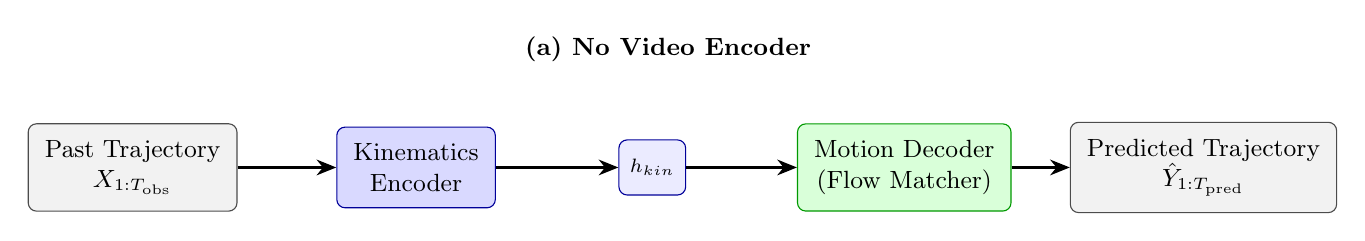
\begin{tikzpicture}
  \node[io]  (x)   at (0.0,0)  {Past Trajectory\\$X_{1:T_{\mathrm{obs}}}$};
  \node[kin] (enc) at (3.6,0)  {Kinematics\\Encoder};
  \node[vec] (h)   at (6.6,0)  {$h_{kin}$};
  \node[dec] (dec) at (9.8,0)  {Motion Decoder\\(Flow Matcher)};
  \node[io]  (y)   at (13.6,0) {Predicted Trajectory\\$\hat{Y}_{1:T_{\mathrm{pred}}}$};

  \draw[arrow] (x)   -- (enc);
  \draw[arrow] (enc) -- (h);
  \draw[arrow] (h)   -- (dec);
  \draw[arrow] (dec) -- (y);

  \node[title] at ($(x)!0.5!(y) + (0,1.5)$) {(a) No Video Encoder};
\end{tikzpicture}
\end{document}
}
    \caption{Kinematics-only baseline of the MoFlow Teacher ($NV$): the past
    trajectory is compressed by a kinematics encoder into $h_{kin}$, and the
    conditional flow-matching decoder regresses the future distribution.
    \label{fig:arch-baseline}}
\end{figure}

% -----------------------------------------------------------------------------
\section{Global Video Encoder Architecture}
\label{sec:global}

The first extension augments the baseline with \emph{global scene-level visual
information}. The rationale is that the past trajectory alone is often
ambiguous: the same kinematics can correspond to different futures depending on
the surrounding structure (walkable areas, obstacles, roads), and the scene
constrains the set of plausible outcomes.

\textbf{Visual feature extraction.} An observed clip $V \in \mathbb{R}^{T_{\mathrm{obs}}
\times H \times W \times 3}$ is processed by a 2D ResNet-18 backbone applied
frame-wise over the $T_{\mathrm{obs}}$ observed frames. This deliberately avoids
3D spatio-temporal convolutions and keeps the temporal alignment with the
trajectory stream explicit. The backbone produces per-frame descriptors
$z_{\mathrm{vid}} \in \mathbb{R}^{T_{\mathrm{obs}} \times D_{\mathrm{raw}}}$
(typically $D_{\mathrm{raw}} = 512$), which are projected into the model
dimension $D$ used throughout the architecture. The backbone is kept small and,
in the current implementation, its features are pre-extracted offline and cached
so that training remains cheap.

\textbf{Fusion with the trajectory stream.} The video tokens are combined with
the trajectory--social tokens $z_{\mathrm{traj}}$ through cross-modal
attention, in which the trajectory tokens act as queries over the visual
tokens:
\begin{equation}
    z_{\mathrm{fused}} = \mathrm{CrossAttention}\big(
        Q = z_{\mathrm{traj}},\; K = z_{\mathrm{vid}},\; V = z_{\mathrm{vid}}\big),
\end{equation}
and the resulting context $z_{\mathrm{ctx}} = \mathrm{Fusion}(z_{\mathrm{traj}},
z_{\mathrm{fused}})$ is injected into the conditional flow-matching decoder, so
that the generated velocity field is explicitly modulated by visual scene
structure: $v_\theta\big(Y^t, t \mid z_{\mathrm{traj}}, z_{\mathrm{vid}}\big)$.
At the scene level no cross-agent masking is required, since the global
representation is shared by all agents.

\begin{figure}[htpb]
    \centering
    \resizebox{\textwidth}{!}{% =====================================================================
%  (b) Global Video Encoder -- scene-level visual context
%  Compile:  pdflatex arch_global_video.tex
% =====================================================================
\documentclass[tikz, border=10pt]{standalone}
\usepackage{amsmath,amssymb}
\usetikzlibrary{arrows.meta, positioning, fit, backgrounds, calc, shapes.geometric}

\tikzset{
  every node/.style={font=\small},
  io/.style   = {rectangle, rounded corners=3pt, draw=gray!60!black,   fill=gray!10,
                 inner sep=6pt, align=center, minimum height=1.0cm},
  kin/.style  = {rectangle, rounded corners=3pt, draw=blue!60!black,   fill=blue!15,
                 inner sep=6pt, align=center, minimum height=1.0cm},
  vid/.style  = {rectangle, rounded corners=3pt, draw=purple!60!black, fill=purple!15,
                 inner sep=6pt, align=center, minimum height=1.0cm},
  fuse/.style = {rectangle, rounded corners=3pt, draw=orange!80!black, fill=orange!20,
                 inner sep=6pt, align=center, minimum height=1.0cm},
  dec/.style  = {rectangle, rounded corners=3pt, draw=green!60!black,  fill=green!15,
                 inner sep=6pt, align=center, minimum height=1.0cm},
  vec/.style  = {rectangle, rounded corners=3pt, draw=blue!60!black,   fill=blue!8,
                 inner sep=4pt, align=center, font=\scriptsize, minimum height=0.7cm},
  vecv/.style = {rectangle, rounded corners=3pt, draw=purple!60!black, fill=purple!8,
                 inner sep=4pt, align=center, font=\scriptsize, minimum height=0.7cm},
  arrow/.style = {-{Stealth[length=2.5mm,width=2mm]}, thick, rounded corners},
  title/.style = {font=\bfseries\small, align=center},
}

\begin{document}
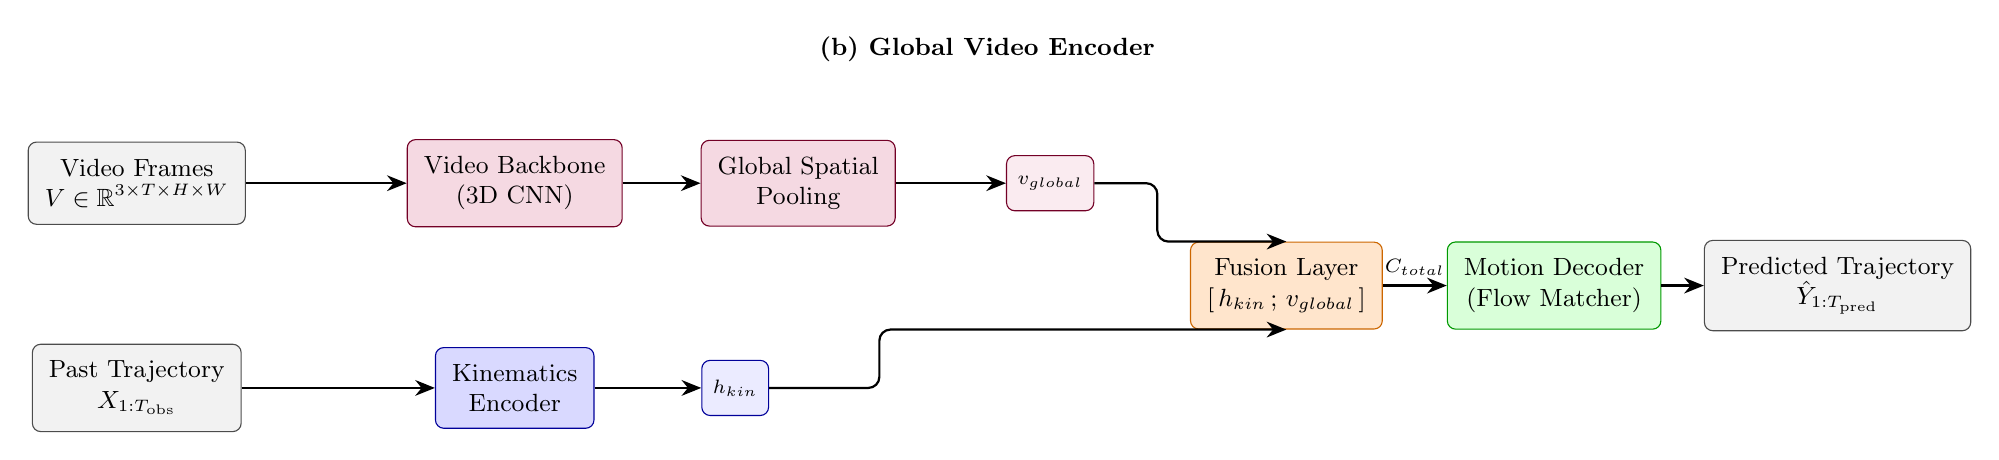
\begin{tikzpicture}
  % ---- kinematics stream (bottom row) ----
  \node[io]  (x)    at (0.0,0.0)   {Past Trajectory\\$X_{1:T_{\mathrm{obs}}}$};
  \node[kin] (kenc) at (4.8,0.0)   {Kinematics\\Encoder};
  \node[vec] (h)    at (7.6,0.0)   {$h_{kin}$};

  % ---- visual stream (top row) ----
  \node[io]   (v)     at (0.0,2.6)  {Video Frames\\$V\in\mathbb{R}^{3\times T\times H\times W}$};
  \node[vid]  (bb)    at (4.8,2.6)  {Video Backbone\\(3D CNN)};
  \node[vid]  (pool)  at (8.4,2.6)  {Global Spatial\\Pooling};
  \node[vecv] (vglob) at (11.6,2.6) {$v_{global}$};

  % ---- fusion + decoder ----
  \node[fuse] (fus) at (14.6,1.3) {Fusion Layer\\$[\,h_{kin}\,;\,v_{global}\,]$};
  \node[dec]  (dec) at (18.0,1.3) {Motion Decoder\\(Flow Matcher)};
  \node[io]   (y)   at (21.6,1.3) {Predicted Trajectory\\$\hat{Y}_{1:T_{\mathrm{pred}}}$};

  % ---- stream arrows ----
  \draw[arrow] (x)    -- (kenc);
  \draw[arrow] (kenc) -- (h);
  \draw[arrow] (v)    -- (bb);
  \draw[arrow] (bb)   -- (pool);
  \draw[arrow] (pool) -- (vglob);

  % ---- merge into fusion ----
  \draw[arrow] (h.east)     -- ++(1.4,0) |- (fus.south);
  \draw[arrow] (vglob.east) -- ++(0.8,0) |- (fus.north);

  \draw[arrow] (fus) -- (dec) node[midway, above, font=\scriptsize] {$C_{total}$};
  \draw[arrow] (dec) -- (y);

  \node[title] at (10.8,4.3) {(b) Global Video Encoder};
\end{tikzpicture}
\end{document}
}
    \caption{Global-video extension ($GV$): the observed clip is embedded by the
    video backbone, pooled into a scene-level token $v_{global}$, and fused with
    the trajectory stream before the flow-matching decoder.
    \label{fig:arch-global}}
\end{figure}

% -----------------------------------------------------------------------------
\section{Results: Baseline vs.\ Global Video Encoder}
\label{sec:results-baseline-global}

Tables \ref{tab:nv-vs-ve} present the per-scene comparison between the
kinematics-only baseline and the global-video-conditioned model on the eight
SDD scenes. Values are scene means over the four reported horizons (labels
given in the metrics glossary in Section~\ref{sec:interpretation}).

\begin{table}[htpb]
    \centering
    \caption{Per-scene comparison, Baseline (``NV'') vs.\ Global Video Encoder
    (``GV''). Scene mean over the reported horizons. Lower is better.
    \label{tab:nv-vs-ve}}
    \small
    \setlength{\tabcolsep}{4pt}
    \begin{tabular}{l rr rr rr rr}
        \toprule
        Scene & \multicolumn{2}{c}{$\mathrm{ADE_{avg}}$}
              & \multicolumn{2}{c}{$\mathrm{FDE_{avg}}$}
              & \multicolumn{2}{c}{$\mathrm{ADE_{min}}$}
              & \multicolumn{2}{c}{$\mathrm{FDE_{min}}$} \\
        \cmidrule(lr){2-3}\cmidrule(lr){4-5}\cmidrule(lr){6-7}\cmidrule(lr){8-9}
              & NV    & GV    & NV    & GV    & NV    & GV    & NV    & GV \\
        \midrule
        bookstore  & 12.960 & 7.981 & 24.058 & 14.843 & 0.675 & 0.529 & 1.071 & 0.744 \\
        coupa      &  6.266 & 6.421 & 11.462 & 11.854 & 0.386 & 0.388 & 0.451 & 0.446 \\
        deathCircle&  7.033 & 7.277 & 12.760 & 13.354 & 0.897 & 0.995 & 1.346 & 1.572 \\
        gates      &  7.642 & 7.964 & 14.126 & 14.675 & 0.849 & 0.828 & 1.149 & 1.106 \\
        hyang      &  8.629 & 7.345 & 15.817 & 13.513 & 0.512 & 0.491 & 0.666 & 0.626 \\
        little     &  6.891 & 6.745 & 12.770 & 12.413 & 0.472 & 0.471 & 0.643 & 0.639 \\
        nexus      &  7.769 & 6.309 & 14.502 & 11.667 & 0.526 & 0.513 & 0.720 & 0.690 \\
        quad       &  7.545 & 7.214 & 13.913 & 13.290 & 0.777 & 0.677 & 0.949 & 0.629 \\
        \bottomrule
    \end{tabular}
\end{table}

\textbf{Summary.} On average-displacement metrics the global video encoder is
strictly better than the kinematics-only baseline in \textbf{5 of 8} scenes
(bookstore, hyang, little, nexus, quad), with the largest gain on \emph{bookstore}
($\mathrm{ADE_{avg}}$: $12.96 \to 7.98$, $-38\%$). The remaining three scenes
(coupa, deathCircle, gates) show only a marginal degradation ($\lesssim +3\%$).
The minimum-error metrics are improved in 6 of 8 scenes for $\mathrm{FDE_{min}}$
(bookstore, coupa, gates, hyang, nexus, quad).

Looking at the scene means over all horizons and scenes, the global branch
reduces $\mathrm{ADE_{avg}}$ from $5.242 \to 4.624$ ($-11.8\%$) and
$\mathrm{FDE_{avg}}$ from $9.346 \to 8.266$ ($-11.6\%$), while the predictive
variance drops by roughly $16\%$ in both $\mathrm{AVar}$ and $\mathrm{FVar}$
(Table~\ref{tab:overall}). Qualitatively, the global-conditioned model tends to
produce futures that respect the walkable structure of the scene
(Figure~\ref{fig:bookstore}).

\begin{figure}[htpb]
    \centering
    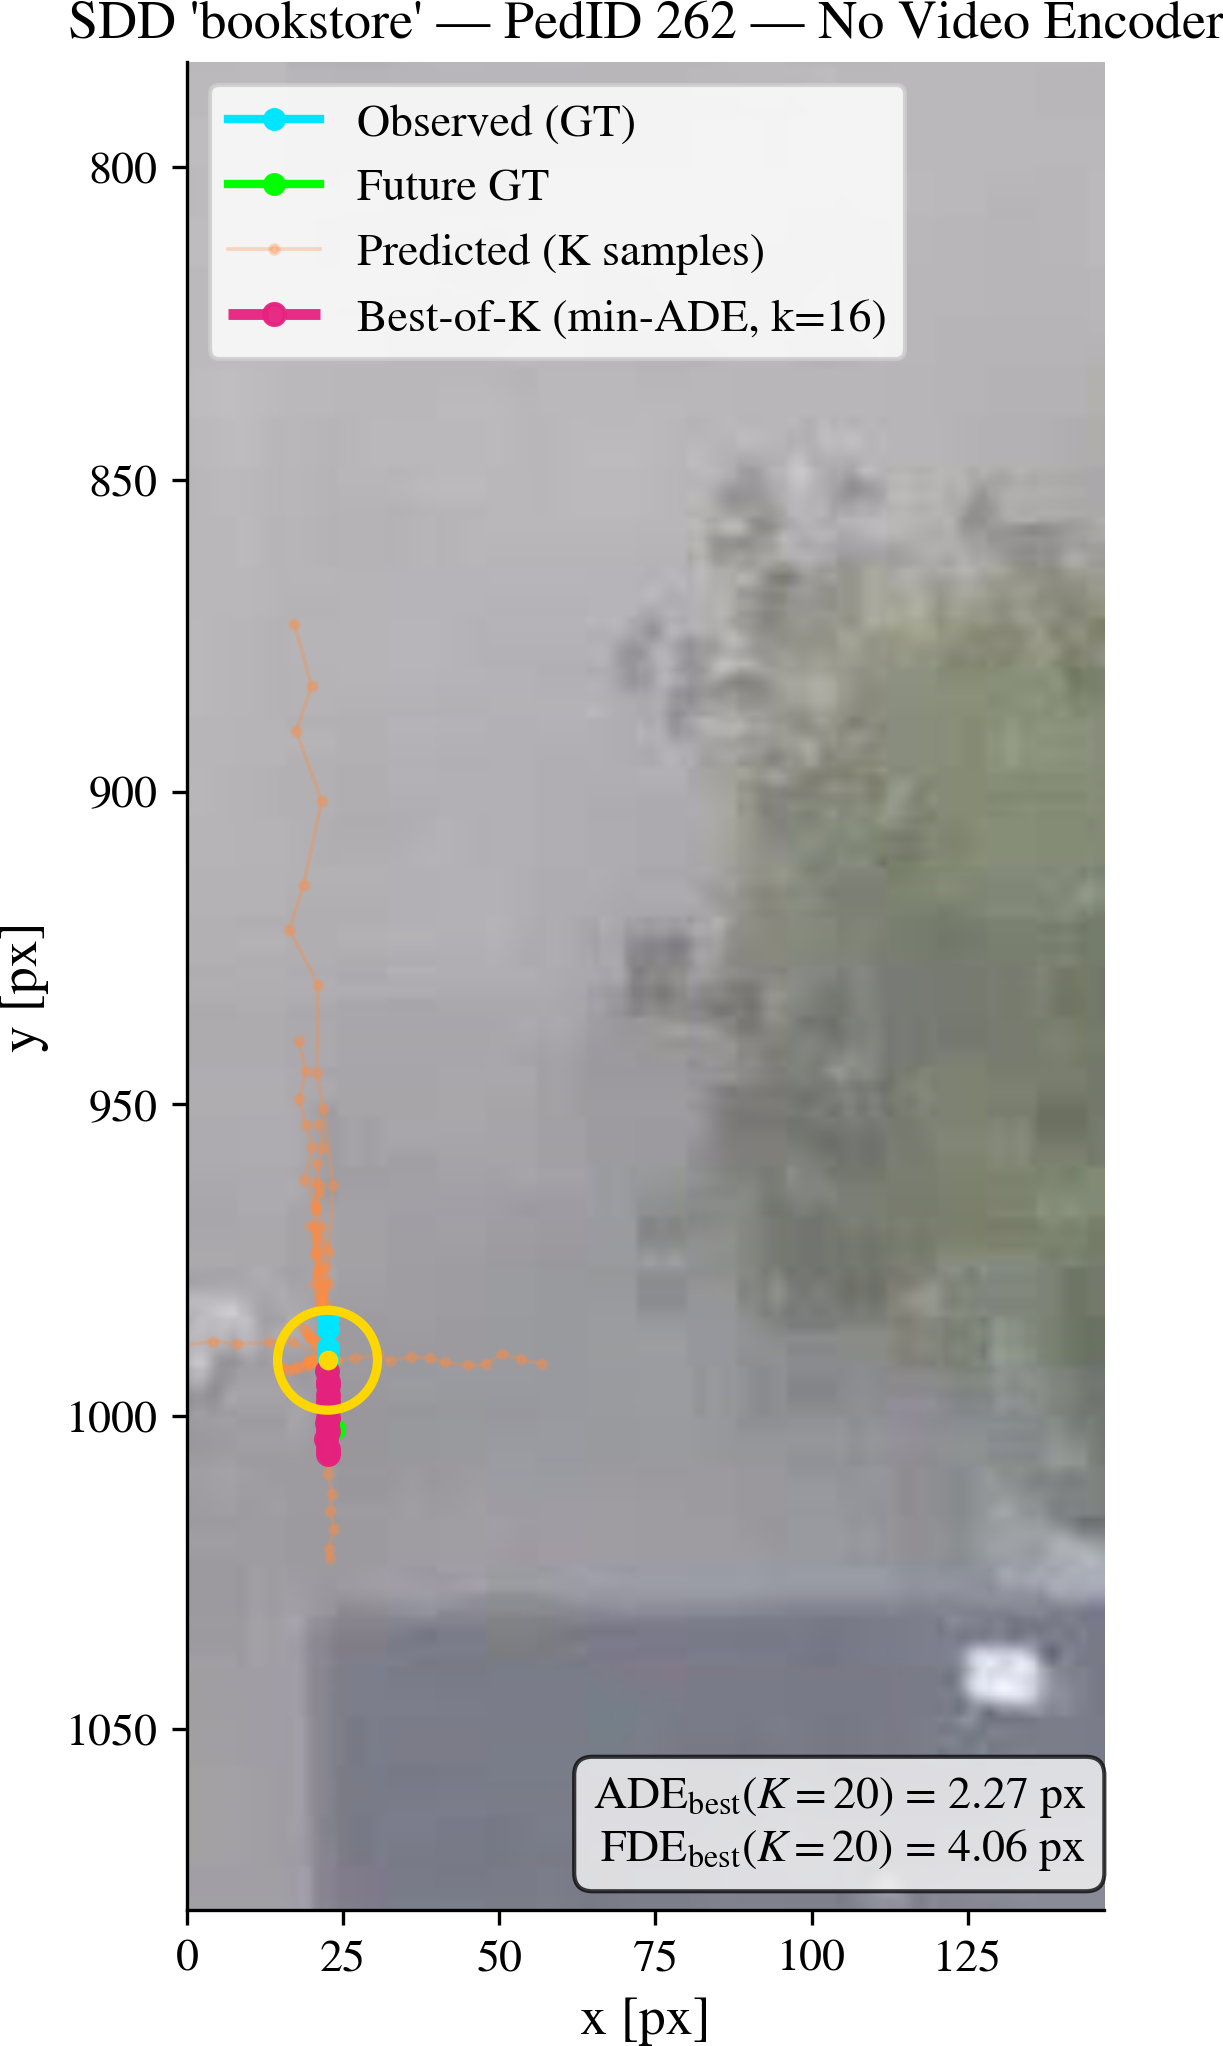
\includegraphics[width=0.32\textwidth]{figures/bookstore_ped262_video1_f5019_no_video.png}
    \hfill
    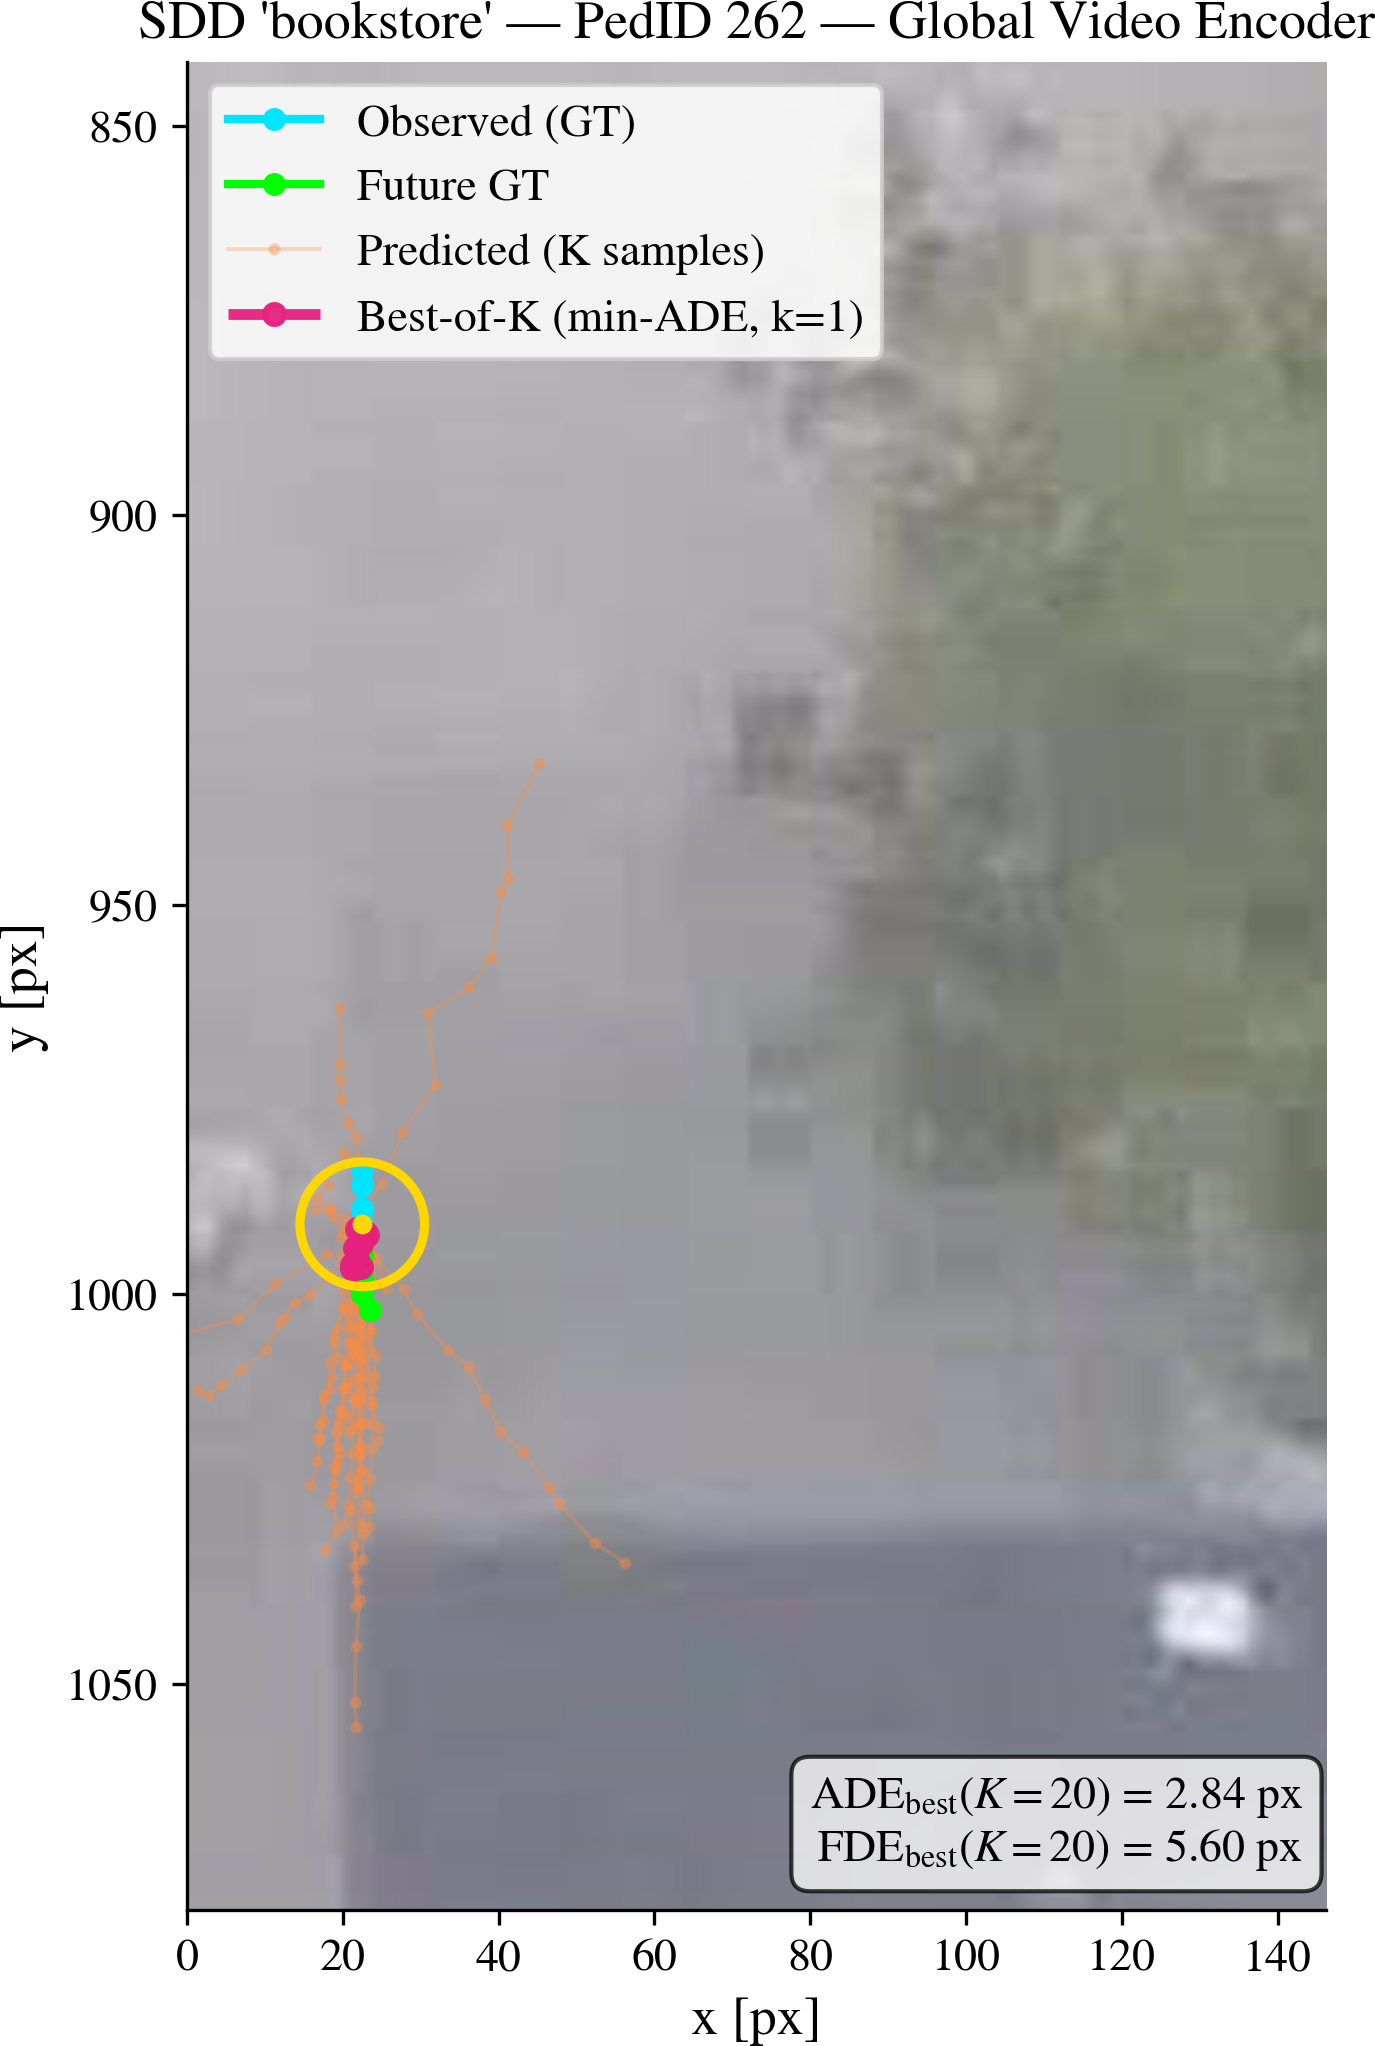
\includegraphics[width=0.32\textwidth]{figures/bookstore_ped262_video1_f5019_global_video.png}
    \hfill
    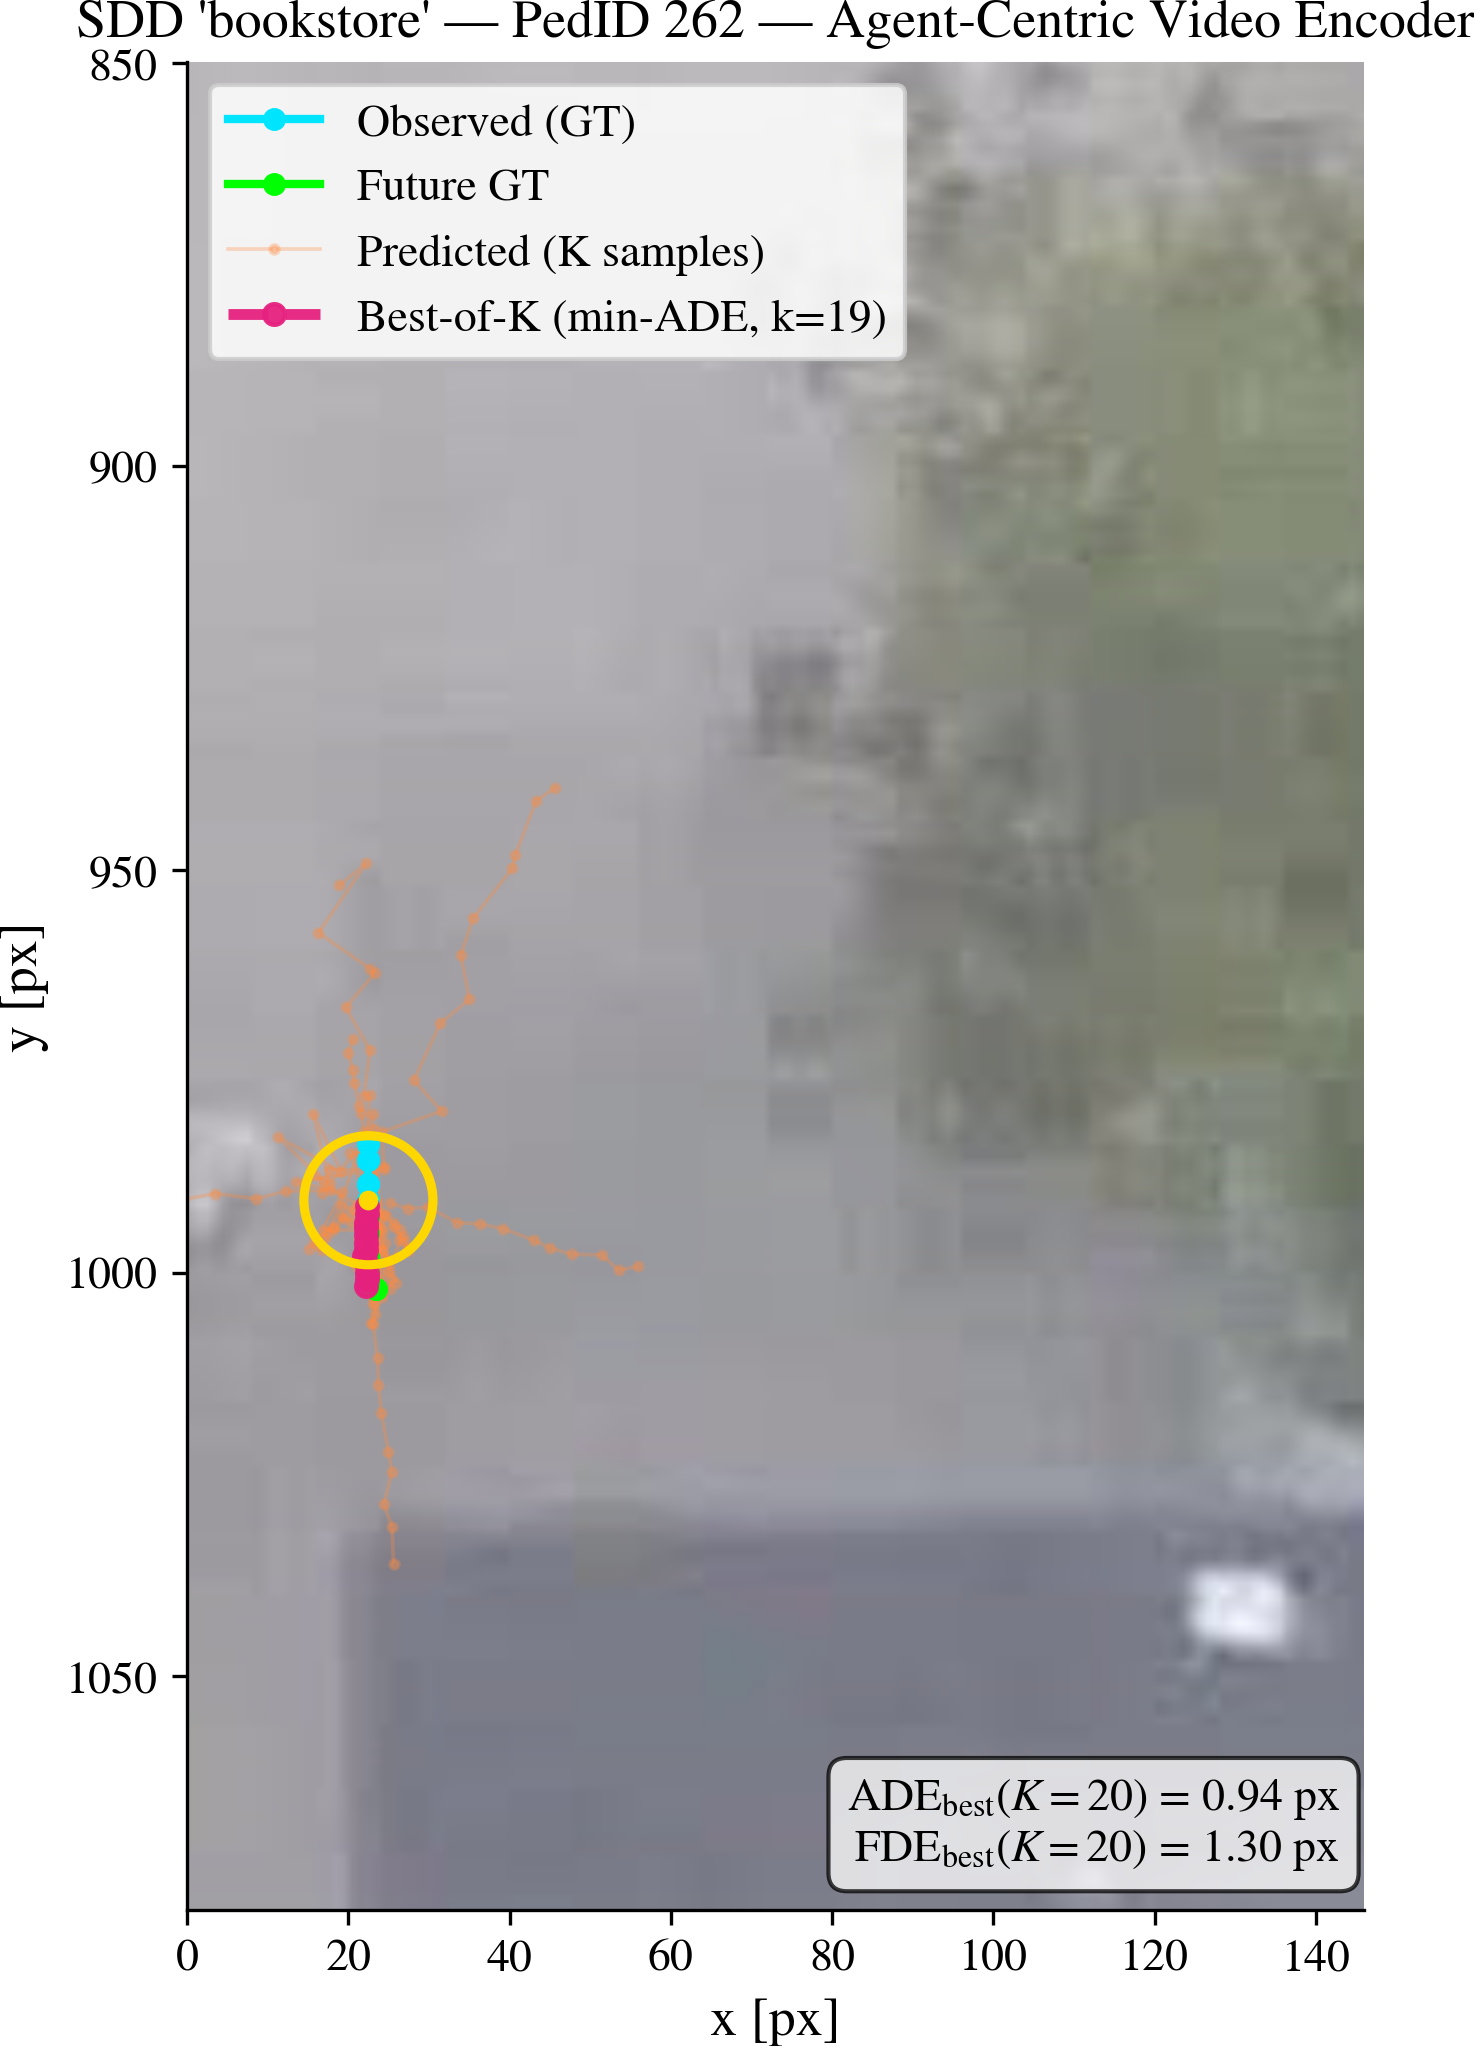
\includegraphics[width=0.32\textwidth]{figures/bookstore_ped262_video1_f5019_agent_centric.png}
    \caption{Qualitative comparison on a bookstore window: no-video, global and
    agent-centric conditioning. In a dense, structured scene the visual branches
    anchor the sampled futures to the walkable area. \label{fig:bookstore}}
\end{figure}

% -----------------------------------------------------------------------------
\section{Agent-Centric Video Encoder Architecture}
\label{sec:agent}

The second extension addresses the local, per-agent visual cues that a global
representation cannot capture: body orientation, posture, immediate neighbours,
and the local obstacles right around the pedestrian. These are precisely the
cues that help to disambiguate \emph{intention}.

\textbf{Per-agent crop extraction.} For each agent $i$ and each observed frame,
the agent's last observed position is projected into pixel space using the
scene's homography (world-to-pixel transform retained by the data loader). A
square patch $P_i^{(t)} \in \mathbb{R}^{h \times w \times 3}$ (default
$64 \times 64$ pixels) is cropped around the projected location, with
zero-padding at image boundaries. Because crops are computed from the same
coordinates that produce the trajectory entries, the agent-ID and temporal-index
arrays remain perfectly aligned with the crop stack --- a strict requirement of
the implementation.

\textbf{Encoding.} The per-agent clip $V_i \in \mathbb{R}^{T_{\mathrm{obs}}
\times 3 \times h \times w}$ is encoded by a shared 2D ResNet-18 (the first
two blocks are kept frozen, with spatial dropout applied after the backbone)
into agent-specific tokens $z_{\mathrm{ag}}^{(i)} \in \mathbb{R}^{T_{\mathrm{obs}}
\times D}$. Thus the output stream has shape $[B, A, T_{\mathrm{obs}}, D]$ and is
subsequently pooled into one token per agent.

\textbf{Tri-modal fusion.} The agent-centric tokens are combined with the two
other modalities through a cascade of two cross-attention steps, in the spirit
of ``flash''-style agents-to-local-then-global attention:
\begin{enumerate}
    \item \emph{Local step (A):} each agent's trajectory token queries its own
          agent-video feature, with a strict \emph{identity mask} so that no
          information leaks between different agents;
    \item \emph{Global step (B):} the locally fused features additionally query
          the global scene tokens from Section~\ref{sec:global}.
\end{enumerate}
Both attention blocks operate in the canonical hidden dimension $D$, keeping
the tensor-shape contract of the architecture unchanged. The final context is
still $[B, A, D]$ and feeds the same motion decoder.

\begin{figure}[htpb]
    \centering
    \resizebox{\textwidth}{!}{% =====================================================================
%  (c) Agent-Centric Video Encoder -- target-conditioned 3D cross-attention
%  Compile:  pdflatex arch_agent_centric.tex
% =====================================================================
\documentclass[tikz, border=10pt]{standalone}
\usepackage{amsmath,amssymb}
\usetikzlibrary{arrows.meta, positioning, fit, backgrounds, calc, shapes.geometric}

\tikzset{
  every node/.style={font=\small},
  io/.style   = {rectangle, rounded corners=3pt, draw=gray!60!black,   fill=gray!10,
                 inner sep=6pt, align=center, minimum height=1.0cm},
  kin/.style  = {rectangle, rounded corners=3pt, draw=blue!60!black,   fill=blue!15,
                 inner sep=6pt, align=center, minimum height=1.0cm},
  vid/.style  = {rectangle, rounded corners=3pt, draw=purple!60!black, fill=purple!15,
                 inner sep=6pt, align=center, minimum height=1.0cm},
  fuse/.style = {rectangle, rounded corners=3pt, draw=orange!80!black, fill=orange!20,
                 inner sep=6pt, align=center, minimum height=1.0cm},
  dec/.style  = {rectangle, rounded corners=3pt, draw=green!60!black,  fill=green!15,
                 inner sep=6pt, align=center, minimum height=1.0cm},
  vec/.style  = {rectangle, rounded corners=3pt, draw=blue!60!black,   fill=blue!8,
                 inner sep=4pt, align=center, font=\scriptsize, minimum height=0.7cm},
  veco/.style = {rectangle, rounded corners=3pt, draw=orange!80!black, fill=orange!8,
                 inner sep=4pt, align=center, font=\scriptsize, minimum height=0.7cm},
  arrow/.style = {-{Stealth[length=2.5mm,width=2mm]}, thick, rounded corners},
  title/.style = {font=\bfseries\small, align=center},
}

\begin{document}
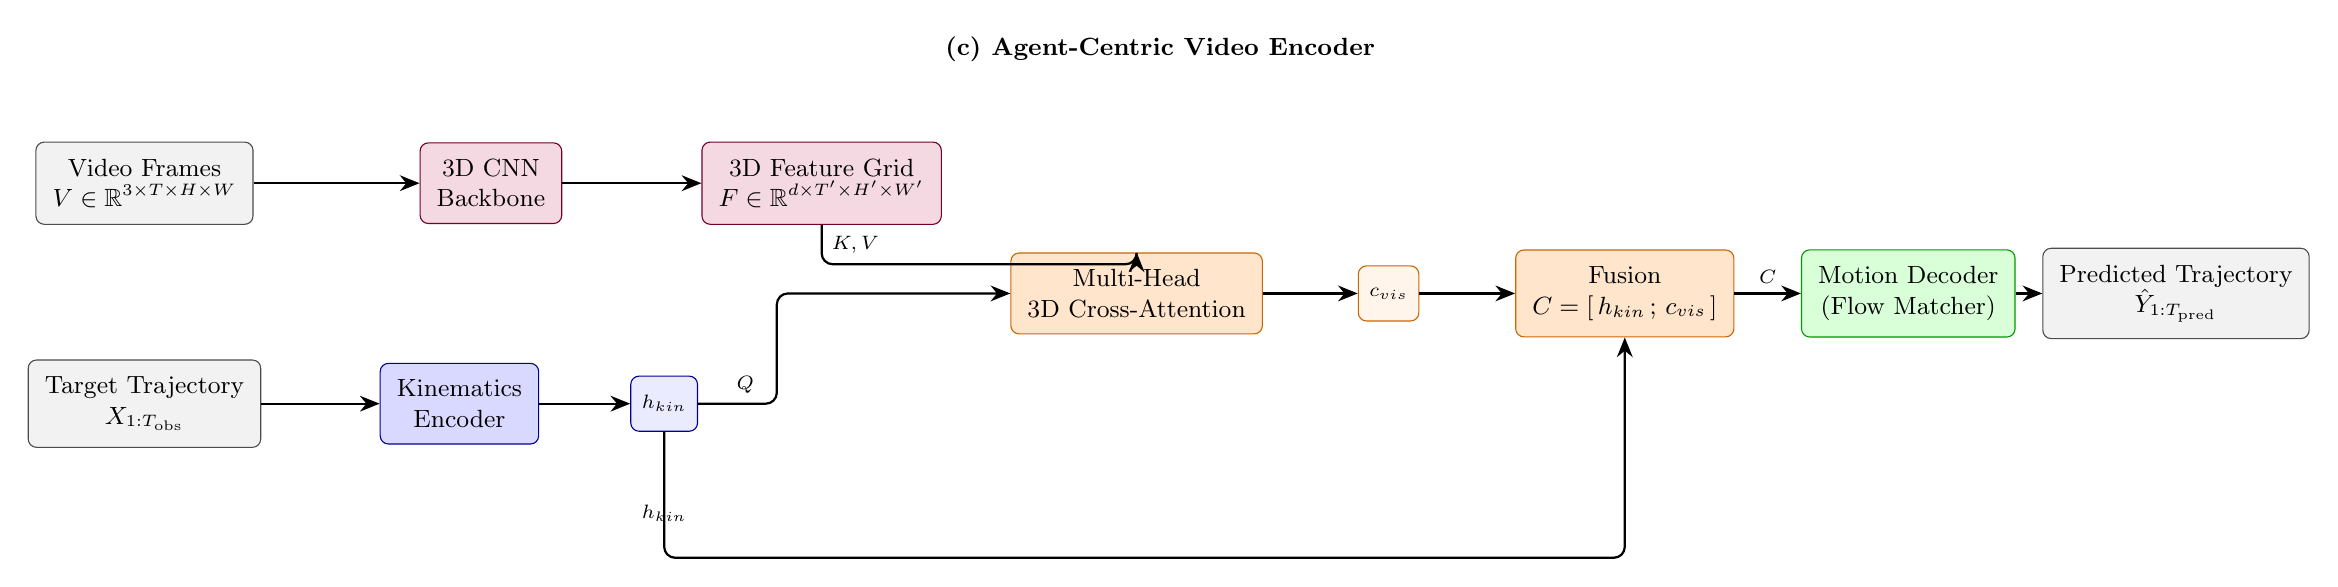
\begin{tikzpicture}
  % ---- target / kinematics stream (bottom row): query ----
  \node[io]  (x)    at (0.0,0.0)  {Target Trajectory\\$X_{1:T_{\mathrm{obs}}}$};
  \node[kin] (kenc) at (4.0,0.0)  {Kinematics\\Encoder};
  \node[vec] (h)    at (6.6,0.0)  {$h_{kin}$};

  % ---- visual stream (top row): keys / values ----
  \node[io]  (v)    at (0.0,2.8)  {Video Frames\\$V\in\mathbb{R}^{3\times T\times H\times W}$};
  \node[vid] (bb)   at (4.4,2.8)  {3D CNN\\Backbone};
  \node[vid] (grid) at (8.6,2.8)  {3D Feature Grid\\$F\in\mathbb{R}^{d\times T'\times H'\times W'}$};

  % ---- attention block + context ----
  \node[fuse] (attn) at (12.6,1.4) {Multi-Head\\3D Cross-Attention};
  \node[veco] (cvis) at (15.8,1.4) {$c_{vis}$};

  % ---- fusion + decoder ----
  \node[fuse] (fus) at (18.8,1.4) {Fusion\\$C=[\,h_{kin}\,;\,c_{vis}\,]$};
  \node[dec]  (dec) at (22.4,1.4) {Motion Decoder\\(Flow Matcher)};
  \node[io]   (y)   at (25.8,1.4) {Predicted Trajectory\\$\hat{Y}_{1:T_{\mathrm{pred}}}$};

  % ---- kinematics + visual stream arrows ----
  \draw[arrow] (x)    -- (kenc);
  \draw[arrow] (kenc) -- (h);
  \draw[arrow] (v)    -- (bb);
  \draw[arrow] (bb)   -- (grid);

  % ---- query / key-value routing into attention ----
  \draw[arrow] (h.east) -- ++(1.0,0)
        node[above, font=\scriptsize, pos=0.6] {$Q$} |- (attn.west);
  \draw[arrow] (grid.south) -- ++(0,-0.5)
        node[right, font=\scriptsize, pos=0.5] {$K,V$} -| (attn.north);

  % ---- attention -> context -> fusion -> decoder -> output ----
  \draw[arrow] (attn) -- (cvis);
  \draw[arrow] (cvis) -- (fus);
  \draw[arrow] (h.south) -- ++(0,-1.6)
        node[below, font=\scriptsize, pos=0.5] {$h_{kin}$} -| (fus.south);
  \draw[arrow] (fus) -- (dec) node[midway, above, font=\scriptsize] {$C$};
  \draw[arrow] (dec) -- (y);

  \node[title] at (12.9,4.5) {(c) Agent-Centric Video Encoder};
\end{tikzpicture}
\end{document}
}
    \caption{Agent-centric extension ($AV$): per-agent crops around the target
    are encoded into local tokens that condition a cross-attention where the
    kinematic state acts as query; the locally fused context $c_{vis}$ is then
    combined with the trajectory stream before the flow-matching decoder.
    \label{fig:arch-agent}}
\end{figure}

% -----------------------------------------------------------------------------
\section{Results: Including Agent-Centric Video}
\label{sec:results-agent}

Adding the agent-centric branch (and keeping the global branch) produces a
markedly different, and more contrasted, pattern.

\begin{table}[htpb]
    \centering
    \caption{Overall means over the eight scenes (scene mean over the reported
    horizons) for the three Teacher models, and relative change $\Delta$ of
    Global (GV) and Agent-Centric (AV) with respect to No-Video (NV). Lower is
    better except where it measures dispersion. \label{tab:overall}}
    \setlength{\tabcolsep}{6pt}
    \begin{tabular}{l rrr rr rr}
        \toprule
        Metric & NV & GV & AV & $\Delta$GV & $\Delta$AV \\
        \midrule
        $\mathrm{ADE_{avg}}$ & 5.242 & 4.624 & 5.834 & $-11.8\%$ & $+11.3\%$ \\
        $\mathrm{FDE_{avg}}$ & 9.346 & 8.266 & 10.482 & $-11.6\%$ & $+12.2\%$ \\
        $\mathrm{ADE_{min}}$ & 0.470 & 0.457 & 0.510 & $-2.8\%$  & $+8.5\%$ \\
        $\mathrm{FDE_{min}}$ & 0.556 & 0.527 & 0.576 & $-5.2\%$  & $+3.6\%$ \\
        $\mathrm{JADE_{min}}$ & 1.229 & 1.120 & 1.096 & $-8.9\%$  & $-10.8\%$ \\
        $\mathrm{JFDE_{min}}$ & 2.058 & 1.826 & 1.697 & $-11.3\%$ & $-17.5\%$ \\
        $\mathrm{AVar}$  & 50.742 & 42.253 & 59.451 & $-16.7\%$ & $+17.2\%$ \\
        $\mathrm{FVar}$  & 133.680 & 112.607 & 158.460 & $-15.8\%$ & $+18.5\%$ \\
        $\mathrm{MASD}$  & 31.295 & 28.178 & 32.644 & $-10.0\%$ & $+4.3\%$ \\
        \bottomrule
    \end{tabular}
\end{table}

The global-video advantage on the \emph{average} metrics is lost: the
agent-centric model is worse than the baseline in 7 of 8 scenes on
$\mathrm{ADE_{avg}}$ (Table~\ref{tab:overall}; e.g.\ \emph{little} $6.891 \to
11.001$, \emph{quad} $7.545 \to 9.986$), and its variance indicators
$\mathrm{AVar}/\mathrm{FVar}$ increase substantially (Table~\ref{tab:overall}).

\begin{table}[htpb]
    \centering
    \caption{Per-scene best-of-$K$ / joint final metrics for the three models.
    Scene mean over the reported horizons. Lower is better.
    \label{tab:min-family}}
    \small
    \setlength{\tabcolsep}{4pt}
    \begin{tabular}{l rrr rrr rrr}
        \toprule
        & \multicolumn{3}{c}{$\mathrm{FDE_{min}}$}
        & \multicolumn{3}{c}{$\mathrm{JADE_{min}}$}
        & \multicolumn{3}{c}{$\mathrm{JFDE_{min}}$} \\
        \cmidrule(lr){2-4}\cmidrule(lr){5-7}\cmidrule(lr){8-10}
        Scene & NV & GV & AV & NV & GV & AV & NV & GV & AV \\
        \midrule
        bookstore  & 1.071 & 0.744 & 0.739 & 2.076 & 1.141 & 1.173 & 3.756 & 1.999 & 1.998 \\
        coupa      & 0.451 & 0.446 & 0.497 & 1.200 & 1.020 & 0.932 & 2.171 & 1.694 & 1.498 \\
        deathCircle& 1.346 & 1.572 & 1.827 & 2.261 & 2.682 & 2.475 & 4.000 & 4.741 & 4.407 \\
        gates      & 1.149 & 1.106 & 1.043 & 2.577 & 2.207 & 2.114 & 4.393 & 3.915 & 3.615 \\
        hyang      & 0.666 & 0.626 & 0.822 & 1.863 & 1.423 & 1.468 & 3.263 & 2.459 & 2.508 \\
        little     & 0.643 & 0.639 & 0.700 & 1.472 & 1.692 & 1.290 & 2.626 & 3.004 & 2.156 \\
        nexus      & 0.720 & 0.690 & 0.489 & 1.387 & 1.280 & 0.992 & 2.519 & 2.257 & 1.663 \\
        quad       & 0.949 & 0.629 & 0.847 & 1.753 & 1.495 & 1.698 & 2.948 & 2.468 & 2.626 \\
        \bottomrule
    \end{tabular}
\end{table}

Strikingly, however, the \emph{best-of-$K$} family paints the opposite picture
(Table~\ref{tab:min-family}): the agent-centric model wins on
$\mathrm{FDE_{min}}$ in 3 of 8 scenes, on $\mathrm{JADE_{min}}$ in 4 of 8, and
on $\mathrm{JFDE_{min}}$ in 5 of 8 scenes, with the clearest gains on
\emph{nexus} ($\mathrm{FDE_{min}}$: $0.720 \to 0.489$, $-32\%$; $\mathrm{JFDE_{min}}$:
$2.519 \to 1.663$, $-34\%$), on \emph{coupa} and on \emph{gates}. The textual
metrics for the agent-centric model are thus split between a deterioration of
the \emph{average} behaviour and an improvement of the \emph{best} behaviour,
which is consistent with the accompanying increase in ensemble variance.

Figure~\ref{fig:arch-combined} summarises the three architectures at a glance.

\begin{figure}[htpb]
    \centering
    \resizebox{\textwidth}{!}{% =====================================================================
%  Combined architecture comparison -- TikZ matrix (vertical stack).
%  Each pipeline is a wide horizontal flow, so stacking at full width keeps
%  the labels legible; the bold (a)/(b)/(c) tags provide the sub-labels.
%  Requires the three sibling PDFs to be compiled first:
%     pdflatex arch_no_video.tex
%     pdflatex arch_global_video.tex
%     pdflatex arch_agent_centric.tex
%     pdflatex arch_combined_all.tex
% =====================================================================
\documentclass[tikz, border=10pt]{standalone}
\usepackage{graphicx}
\usetikzlibrary{matrix, positioning}

\begin{document}
\begin{tikzpicture}
  \matrix (M) [
      matrix of nodes,
      row sep=6mm,
      column sep=5mm,
      nodes={anchor=center, font=\small},
    ] {
      \textbf{(a)} & 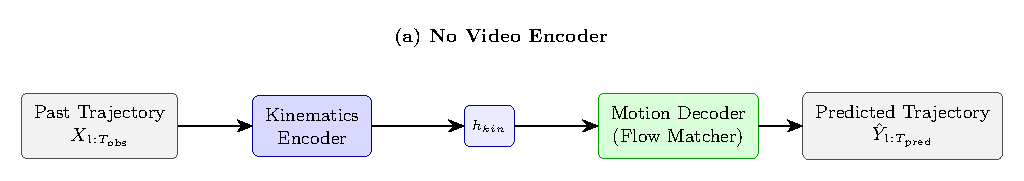
\includegraphics[width=15.5cm]{arch_no_video.pdf} \\
      \textbf{(b)} & 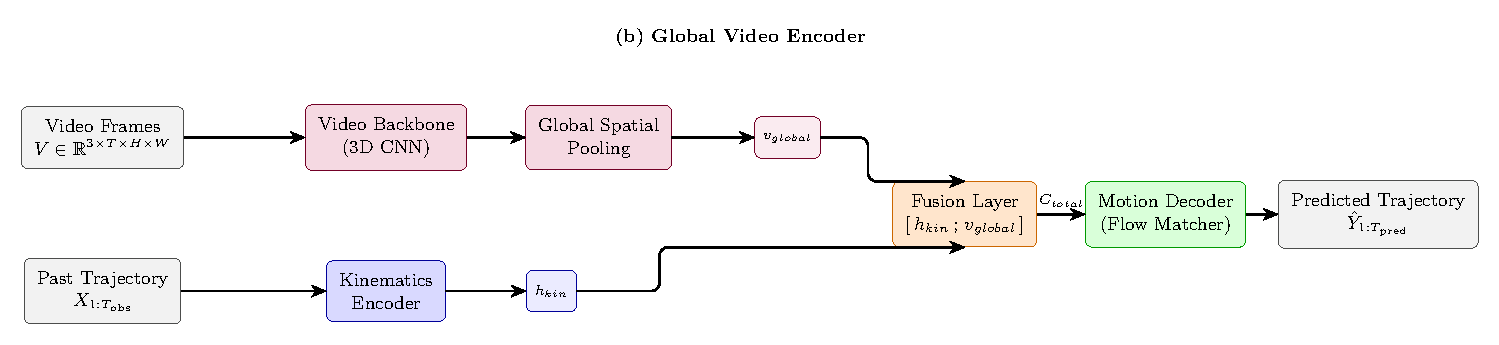
\includegraphics[width=15.5cm]{arch_global_video.pdf} \\
      \textbf{(c)} & 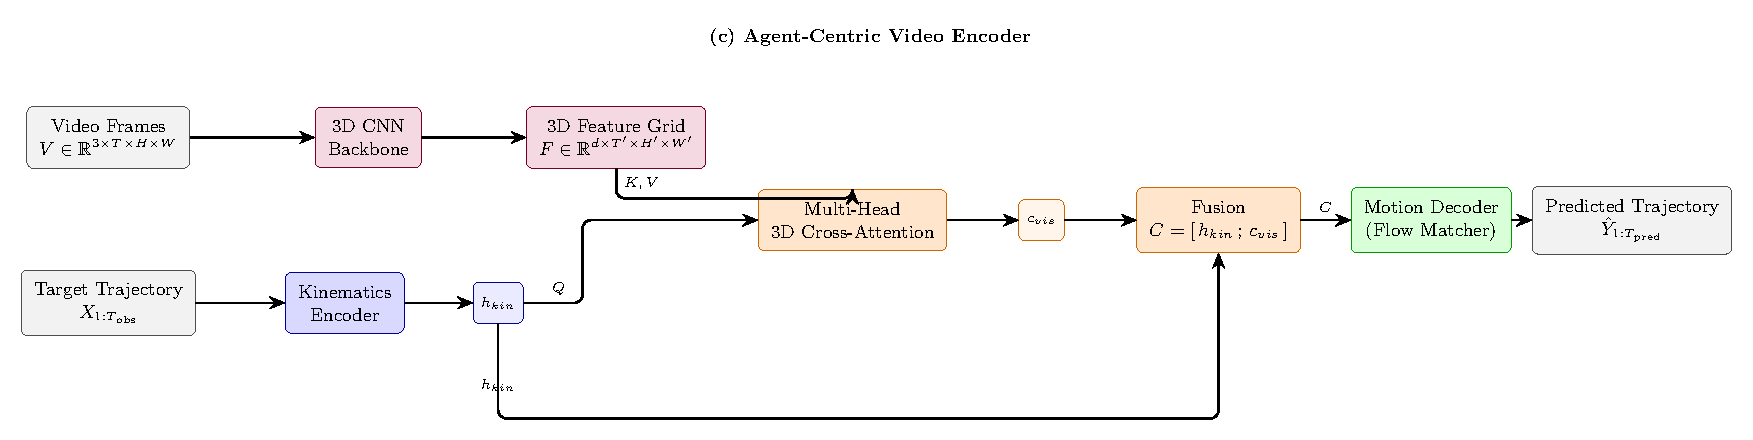
\includegraphics[width=15.5cm]{arch_agent_centric.pdf} \\
    };
\end{tikzpicture}
\end{document}
}
    \caption{The three Teacher architectures compared: (a) kinematics-only
    baseline, (b) global-video, and (c) agent-centric conditioning.
    \label{fig:arch-combined}}
\end{figure}

% -----------------------------------------------------------------------------
\section{Interpretation of Results}
\label{sec:interpretation}

To interpret the per-scene differences reported above, the intrinsic conditions
of each scene were quantified directly from the raw SDD annotations: the crowd
density (mean and peak number of simultaneously visible pedestrians), the
intensity of pairwise proximity between pedestrians (mean number of close
pairs per frame at 25 px and 50 px), the presence and activity of
non-pedestrian entities (bikers, skaters, carts, cars, buses), and the mean
per-frame displacement of the agents. Table~\ref{tab:complexity} summarises
these statistics; they serve in this section as the observed scene facts
against which the behaviour of the three models is interpreted.

\begin{table}[htpb]
    \centering
    \caption{Scene-complexity statistics aggregated over all recordings of each
    SDD scene. $\overline{A}_{\mathrm{ped}}$/$A_{\max}$: mean/peak active
    pedestrians per frame; $\mathrm{pairs}_{<d}$: mean number of pedestrian
    pairs per frame with centres closer than $d$~px; $n_{\mathrm{NP}}$: distinct
    non-pedestrian tracks; $\overline{A}_{\mathrm{NP}}$: mean active
    non-pedestrian agents per frame; $\overline{v}$: mean per-frame step length
    (px/frame); $\kappa$: fraction of the scene footprint covered by pedestrian
    boxes.\label{tab:complexity}}
    \small
    \setlength{\tabcolsep}{4pt}
    \begin{tabular}{l rrr rr rrr}
        \toprule
        Scene & $\overline{A}_{\mathrm{ped}}$ & $A_{\max}$
              & $\mathrm{pairs}_{<25}$ & $\mathrm{pairs}_{<50}$
              & $n_{\mathrm{NP}}$ & $\overline{A}_{\mathrm{NP}}$ & $\overline{v}$ & $\kappa$ \\
        \midrule
        bookstore   & 71.5  & 116 & 8.4  & 28.2 & 363 & 41.5 & 0.83 & 0.092 \\
        coupa       & 40.5  &  70 & 2.3  & 17.5 &  85 &  9.9 & 0.75 & 0.058 \\
        deathCircle & 56.6  & 133 & 9.5  & 29.1 &1272 &113.9 & 1.26 & 0.040 \\
        gates       & 48.5  & 164 & 5.2  & 16.0 & 386 & 63.7 & 1.28 & 0.055 \\
        hyang       & 120.6 & 253 & 31.2 & 92.6 & 370 & 52.5 & 0.84 & 0.079 \\
        little      & 18.0  &  58 & 1.2  &  4.7 & 228 & 25.1 & 1.39 & 0.024 \\
        nexus       & 100.1 & 256 & 22.5 & 74.8 & 270 & 55.7 & 0.57 & 0.094 \\
        quad        & 48.1  &  51 & 6.3  & 23.0 &   6 &  8.0 & 0.92 & 0.024 \\
        \bottomrule
    \end{tabular}
\end{table}

\subsection{Crowd density and social interactions}

\emph{hyang} and \emph{nexus} are by far the most crowded scenes: they average
\textbf{120.6} and \textbf{100.1} simultaneously active pedestrians per frame,
peaking at 253 and 256, and exhibit the largest proximity loads, with 31.2 and
22.5 close pedestrian pairs per frame within 25 px and 92.6 and 74.8 pairs
within 50 px, respectively. \emph{bookstore} is the densest in per-area terms
(0.047 active pedestrians per $10^3$ px$^2$, largest of all scenes) and, with
\emph{nexus}, has the highest spatial coverage ($\kappa \approx 0.09$). In
these interaction-rich scenes both video branches systematically improve over
the kinematics-only baseline, but along \emph{different} metrics.

The global branch produces its largest average gains precisely here:
$\mathrm{ADE_{avg}}$ drops from 8.63 to 7.35 on \emph{hyang} ($-15\%$), from
7.77 to 6.31 on \emph{nexus} ($-19\%$), and from 12.96 to 7.98 on
\emph{bookstore} ($-38\%$), where the predictive variance collapses as well
($\mathrm{AVar}$: 227.8 $\to$ 107.5, $-53\%$). We attribute this to the global
descriptor acting as a \emph{structural prior} that captures the walkable
layout of these geometrically constrained scenes: it narrows the generated
ensemble around physically admissible regions and reduces the variance of the
forecast by roughly $16\%$ overall, exactly the behaviour expected of a
conditioning signal that lowers the entropy of the future distribution.

Crowded frames are, however, precisely where a {\em single pooled} scene
embedding is most diluted: in a frame containing hundreds of agents, each
individual contributes a negligible fraction of the global descriptor, which
therefore encodes ``the scene'' but nothing about a \emph{specific} agent.
This wash-out is visible in the extreme-error statistics: on \emph{nexus} the
global model's minimum metrics ($\mathrm{FDE_{min}} = 0.690$,
$\mathrm{JFDE_{min}} = 2.257$) are superseded by the agent-centric model's
$0.489$ ($\mathrm{FDE_{min}}$, $-32\%$ vs.\ baseline) and $1.663$
($\mathrm{JFDE_{min}}$, $-34\%$), with $\mathrm{JADE_{min}} = 0.992$ the best
of all variants. The agent-centric branch instead bases its
representation on each agent's \emph{own} crop through target-conditioned
cross-attention with strict identity masking; it consequently maintains a sharp,
focused prediction distribution even at peak crowd density, because the visual
evidence attached to the query agent is isolated rather than averaged away.
On \emph{hyang} the same pattern holds for the joint final metrics: the
agent-centric $\mathrm{JFDE_{min}} = 2.508$ is within $2\%$ of the global model
(2.459) and far below the baseline (3.263, $-23\%$).

The converse is equally instructive. \emph{little}, the least dense scene
(18.0 active pedestrians, $0.006\,\mathrm{px}^{-2}$ density, only 1.2 close
pairs per frame) and the fastest one ($\overline v = 1.39$ px/frame), is the
only scene where the agent-centric model degrades the average error markedly
($\mathrm{ADE_{avg}}$: 6.89 $\to$ 11.00, $+60\%$). When pedestrians are sparse
and move quickly, crops frequently miss the target or are dominated by fast
occluders, so the local representation injects noise on average --- yet the
same branch still yields the best $\mathrm{JFDE_{min}}$ of any model
($2.156$, $-18\%$ vs.\ baseline), confirming that its mode sharpness persists
whenever the crop is on target.

\subsection{The role of heterogeneous and dynamic non-pedestrian obstacles}

Every scene contains substantial non-pedestrian traffic, but its composition
differs sharply. \emph{deathCircle} is extreme: \textbf{1{,}272} non-pedestrian
tracks, among them \textbf{914} bikers joined by 106 cars, 128 carts, 106
skaters and 18 buses, with \textbf{113.9} such agents active per frame --- more
than the 56.6 pedestrians --- and fast, volatile motion ($\overline v = 1.26$,
std.\ 2.23). \emph{nexus} is automotive rather than two-wheeled: 119 cars and
30 buses among its 270 non-pedestrian tracks, moving slowly (0.57 px/frame,
the most congested scene) with up to 256 pedestrians present. \emph{gates} and
\emph{little} are biker-dominated (315 and 218 biker tracks), and the latter
hosts the fastest pedestrian motion.

Dynamic obstacles cannot be captured by a {\em static} scene prior: a biker or
vehicle traverses the field of view, so any spatially pooled descriptor mixes
past and present occupancy and the ``walkable area'' changes at the frame
rate. This is the clearest failure mode of the global branch. On
\emph{deathCircle} every model degrades, but the global variant is worst
precisely on the min metrics ($\mathrm{FDE_{min}}$ 1.572 vs.\ 1.346 for the
baseline; $\mathrm{JFDE_{min}}$ 4.741, the largest of all three), consistent
with a pooled descriptor saturated by moving clutter. The agent-centric model
recovers here by conditioning on the \emph{current} free corridor around each
target, which lets the flow matcher tighten its best-of-$K$ modes around
feasible pathways and steer them away from collisions (Figure~\ref{fig:nexus}).
The evidence spans the
obstacle-rich scenes: on \emph{nexus} the automotive mix coexists with the
largest min-family gains ($\mathrm{FDE_{min}}$ $-32\%$,
$\mathrm{JFDE_{min}}$ $-34\%$); on \emph{gates} with 315 bikers the
agent-centric model is the only variant to improve $\mathrm{FDE_{min}}$
(1.149 $\to$ 1.043, $-9\%$) and $\mathrm{JADE_{min}}$ (2.577 $\to$ 2.114,
$-18\%$); on \emph{coupa}, despite its light traffic (85 non-pedestrian
tracks), it cuts $\mathrm{JADE_{min}}$ by $22\%$ and $\mathrm{JFDE_{min}}$ by
$31\%$.

\emph{deathCircle} also exposes the boundary of the agent-centric design:
under such extreme dynamic load, crops are frequently saturated by
high-speed distractors, and the average error inflates ($\mathrm{FDE_{avg}}$
$+16\%$) as does $\mathrm{FDE_{min}}$ ($+36\%$). Yet the branch still keeps the
{\em best} joint-final error among the video variants there (4.407 vs.\ 4.741
for the global model), i.e. at least one generated mode remains on a feasible
trajectory even when the pooled scene descriptor is most diluted. The same
mean-vs.\ mode split is seen on \emph{little} (worst average, best
$\mathrm{JFDE_{min}}$), underlining that per-agent visual focus protects the
extremes of the distribution even when it cannot protect its mean.

\subsection{Trade-off between the global prior and the agent-centric focus}

The two video branches are complementary rather than redundant, acting on
different parts of the forecast distribution. The \textbf{global model acts as
a variance-reducing structural prior}: it improves the average metrics in 5 of
8 scenes, wins $5/8$ scenes on each of $\mathrm{AVar}$ and $\mathrm{FVar}$, and
reduces both by $\sim 16\%$ overall. Its agent-agnostic, pooled descriptor
regularises the ensemble around walkable structure --- lowering the entropy of
the generative field --- without committing to any single agent; consequently
its best-of-$K$ tail is only moderately sharpened ($\mathrm{FDE_{min}}$ is best
in 4/8 scenes, $\mathrm{JADE_{min}}$ in 3/8), because no per-agent evidence
exists to anchor a particular mode.

The \textbf{agent-centric model is a mode specialist}. By attending only to the
target's own crop (identity-masked), it produces sharper commitments: it
achieves the best $\mathrm{FDE_{min}}$ in 3/8 scenes, $\mathrm{JADE_{min}}$ in
4/8 and $\mathrm{JFDE_{min}}$ in 5/8, and improves $\mathrm{JADE_{min}}$ and
$\mathrm{JFDE_{min}}$ overall by $-10.8\%$ and $-17.5\%$ --- the largest
min-family reductions of any variant. The cost is explicit in the statistics:
ensemble variance grows ($\mathrm{AVar}$ $+17.2\%$, $\mathrm{FVar}$ $+18.5\%$)
and the average errors worsen ($\mathrm{ADE_{avg}}$ $+11.3\%$). Restricting
attention to one agent removes the shared social support that each sample
otherwise receives, so individual modes become sharper while the global spread
--- and with it the mean error --- grows.

Taken together, the global branch shapes the \emph{centre and dispersion} of
the predicted distribution, whereas the agent-centric branch shapes its
\emph{feasible-mode coverage}. The interaction between the two is
scene-conditional: in static, geometrically dense scenes such as
\emph{bookstore} the global prior dominates; in sparse, fast scenes such as
\emph{little} neither branch improves the mean, yet the agent-centric model
preserves a good mode; and in congested corridors such as \emph{nexus} and
\emph{hyang} the two streams contribute on complementary metrics. This suggests
that a merged configuration which keeps the global prior for stability and the
agent-centric focus for mode sharpness, with an attention weighting conditioned
on scene complexity, is the most promising direction to explore next.

\subsection{Status and limitations}

These interpretations remain \emph{preliminary}: each model was trained with a
single configuration and a single seed on pre-extracted visual features, so the
magnitudes of the reported differences must be read as indicative rather than
as statistically established. The scene statistics are aggregated over all
frames of all recordings of a scene at the raw-annotation rate; speeds are
reported in pixels per frame and the pair thresholds (25/50 px) are heuristic.
\emph{quad} rests on a very small sample (four recordings, 509 frames, 24
pedestrian and 6 non-pedestrian tracks) and its results should be treated with
caution.

\begin{figure}[htpb]
    \centering
    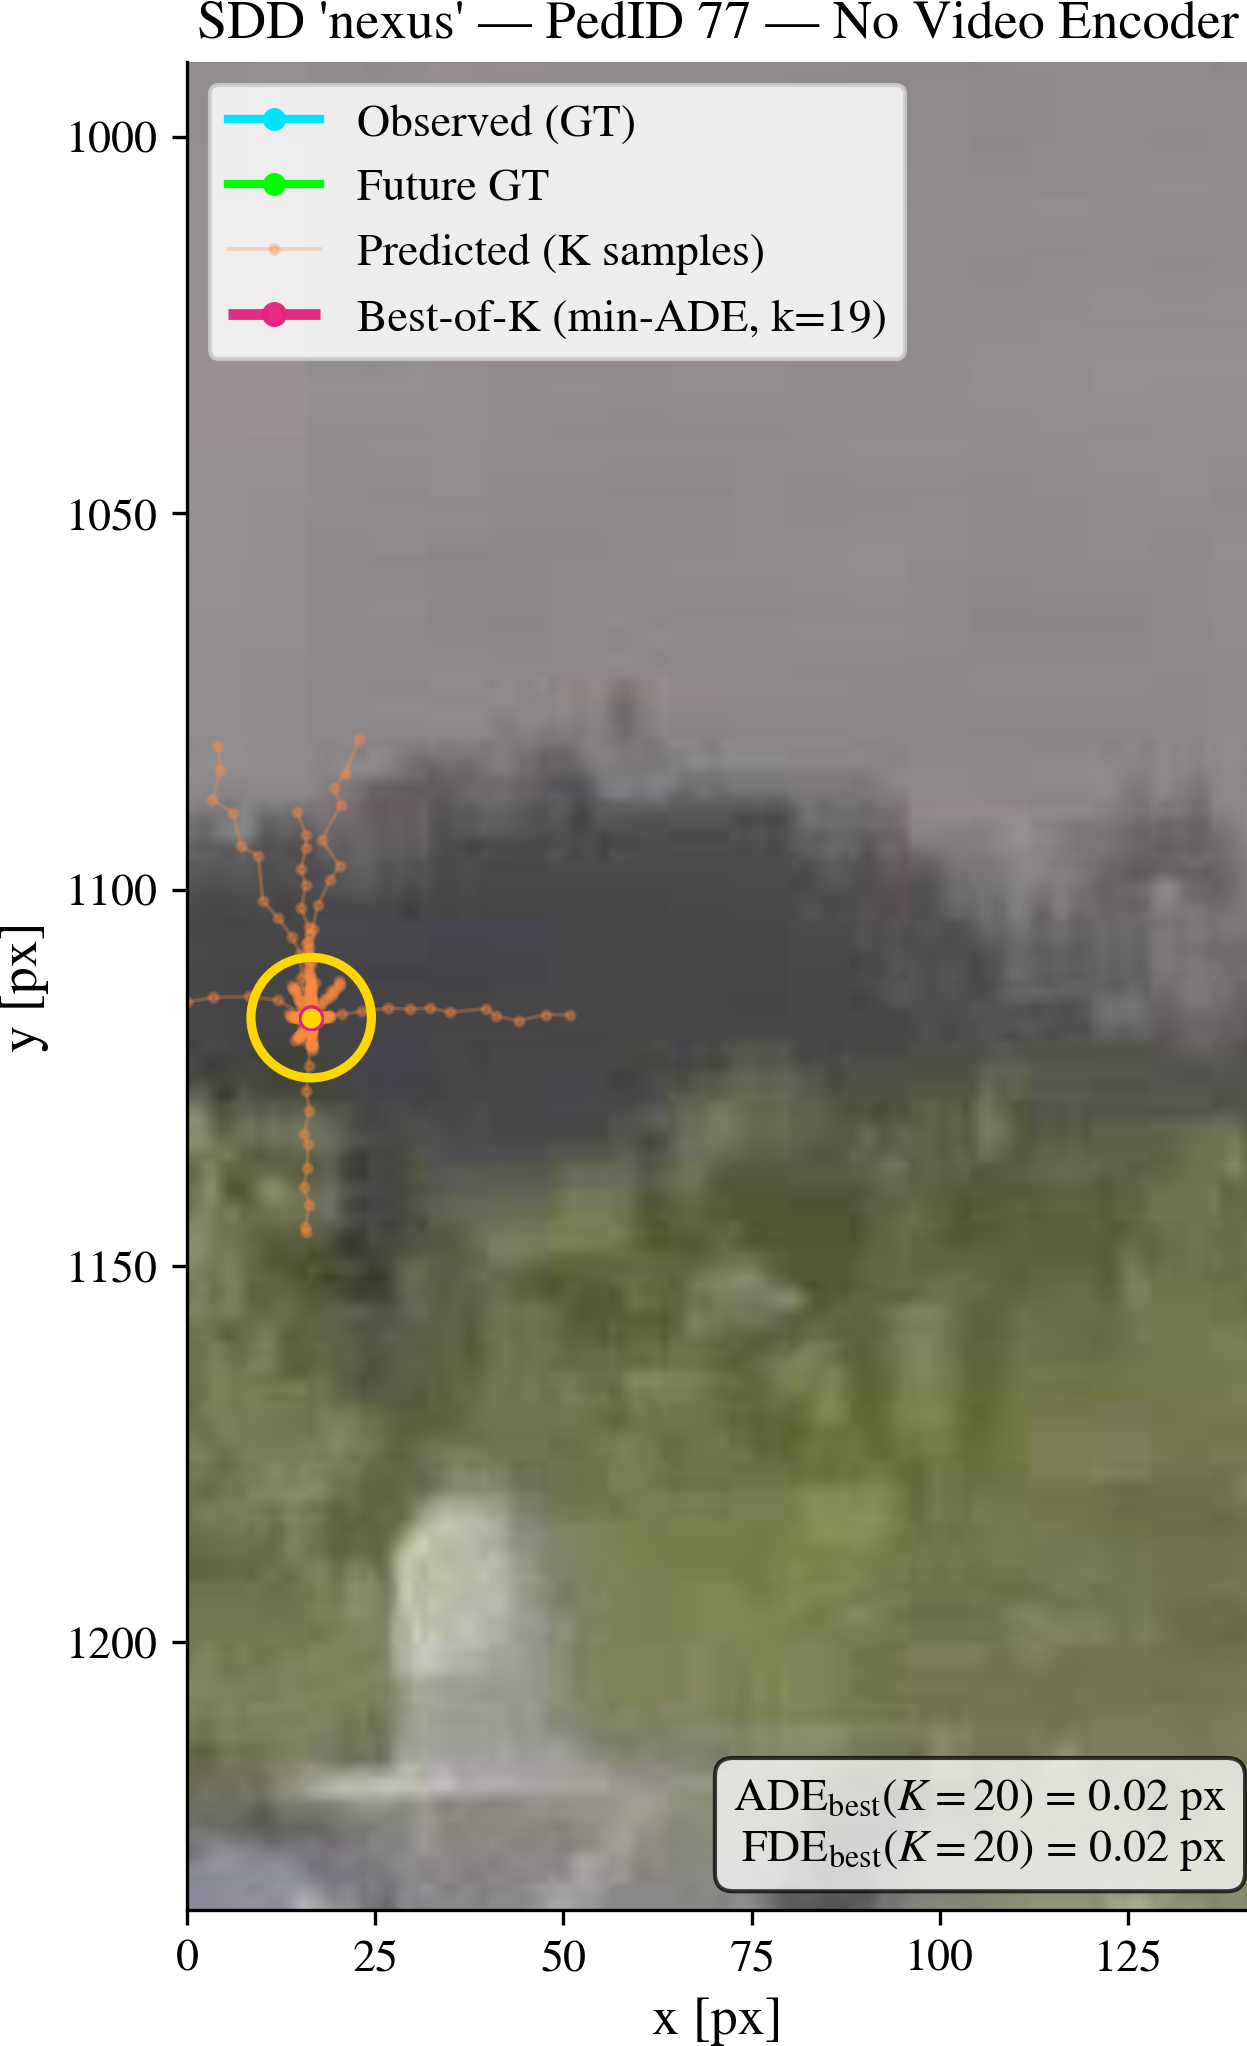
\includegraphics[width=0.32\textwidth]{figures/nexus_ped77_video9_f2519_no_video.png}
    \hfill
    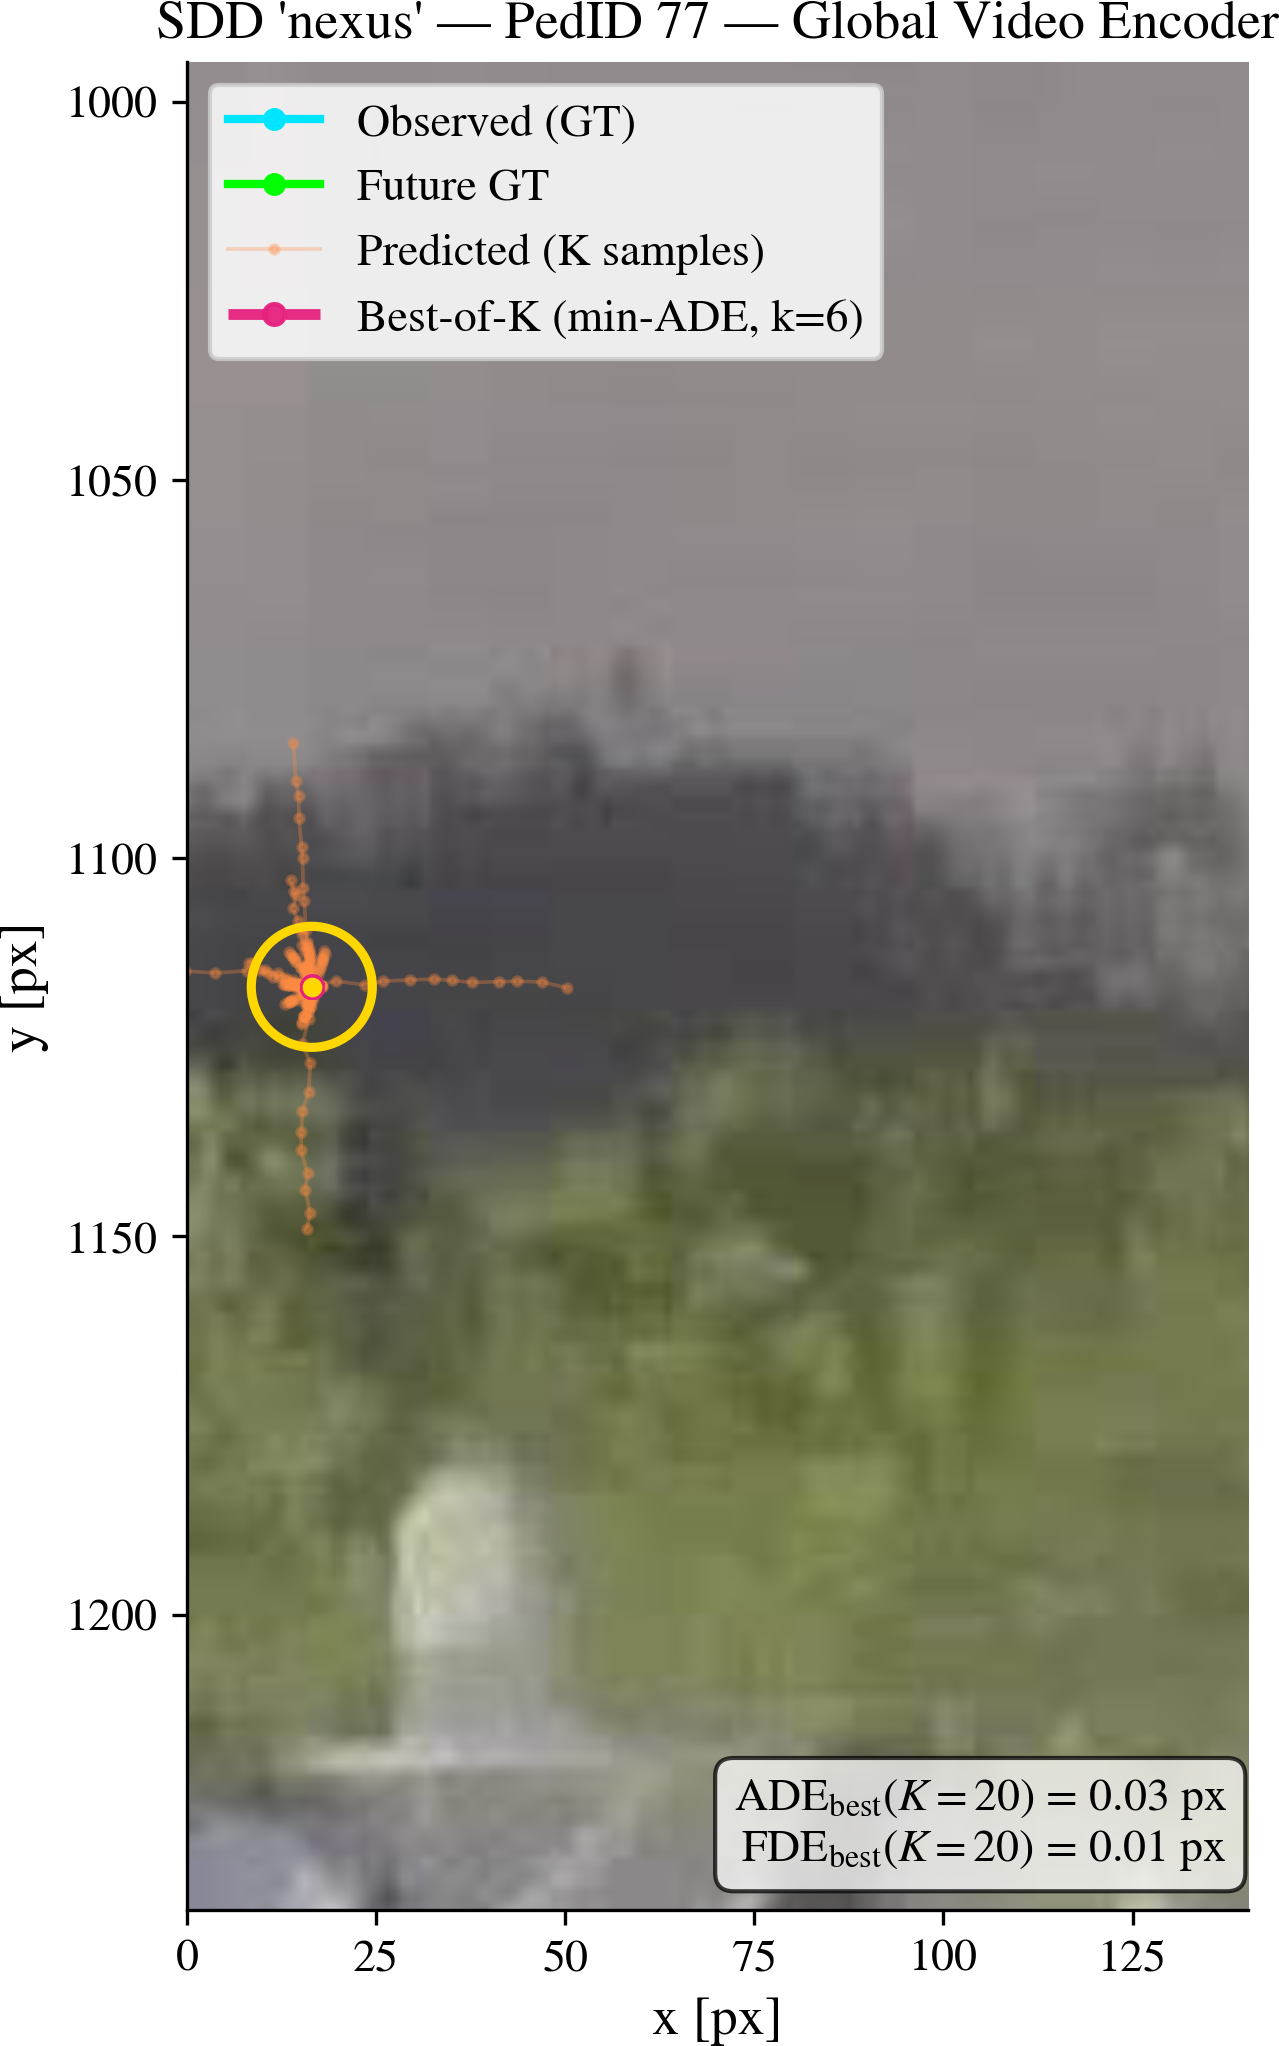
\includegraphics[width=0.32\textwidth]{figures/nexus_ped77_video9_f2519_global_video.png}
    \hfill
    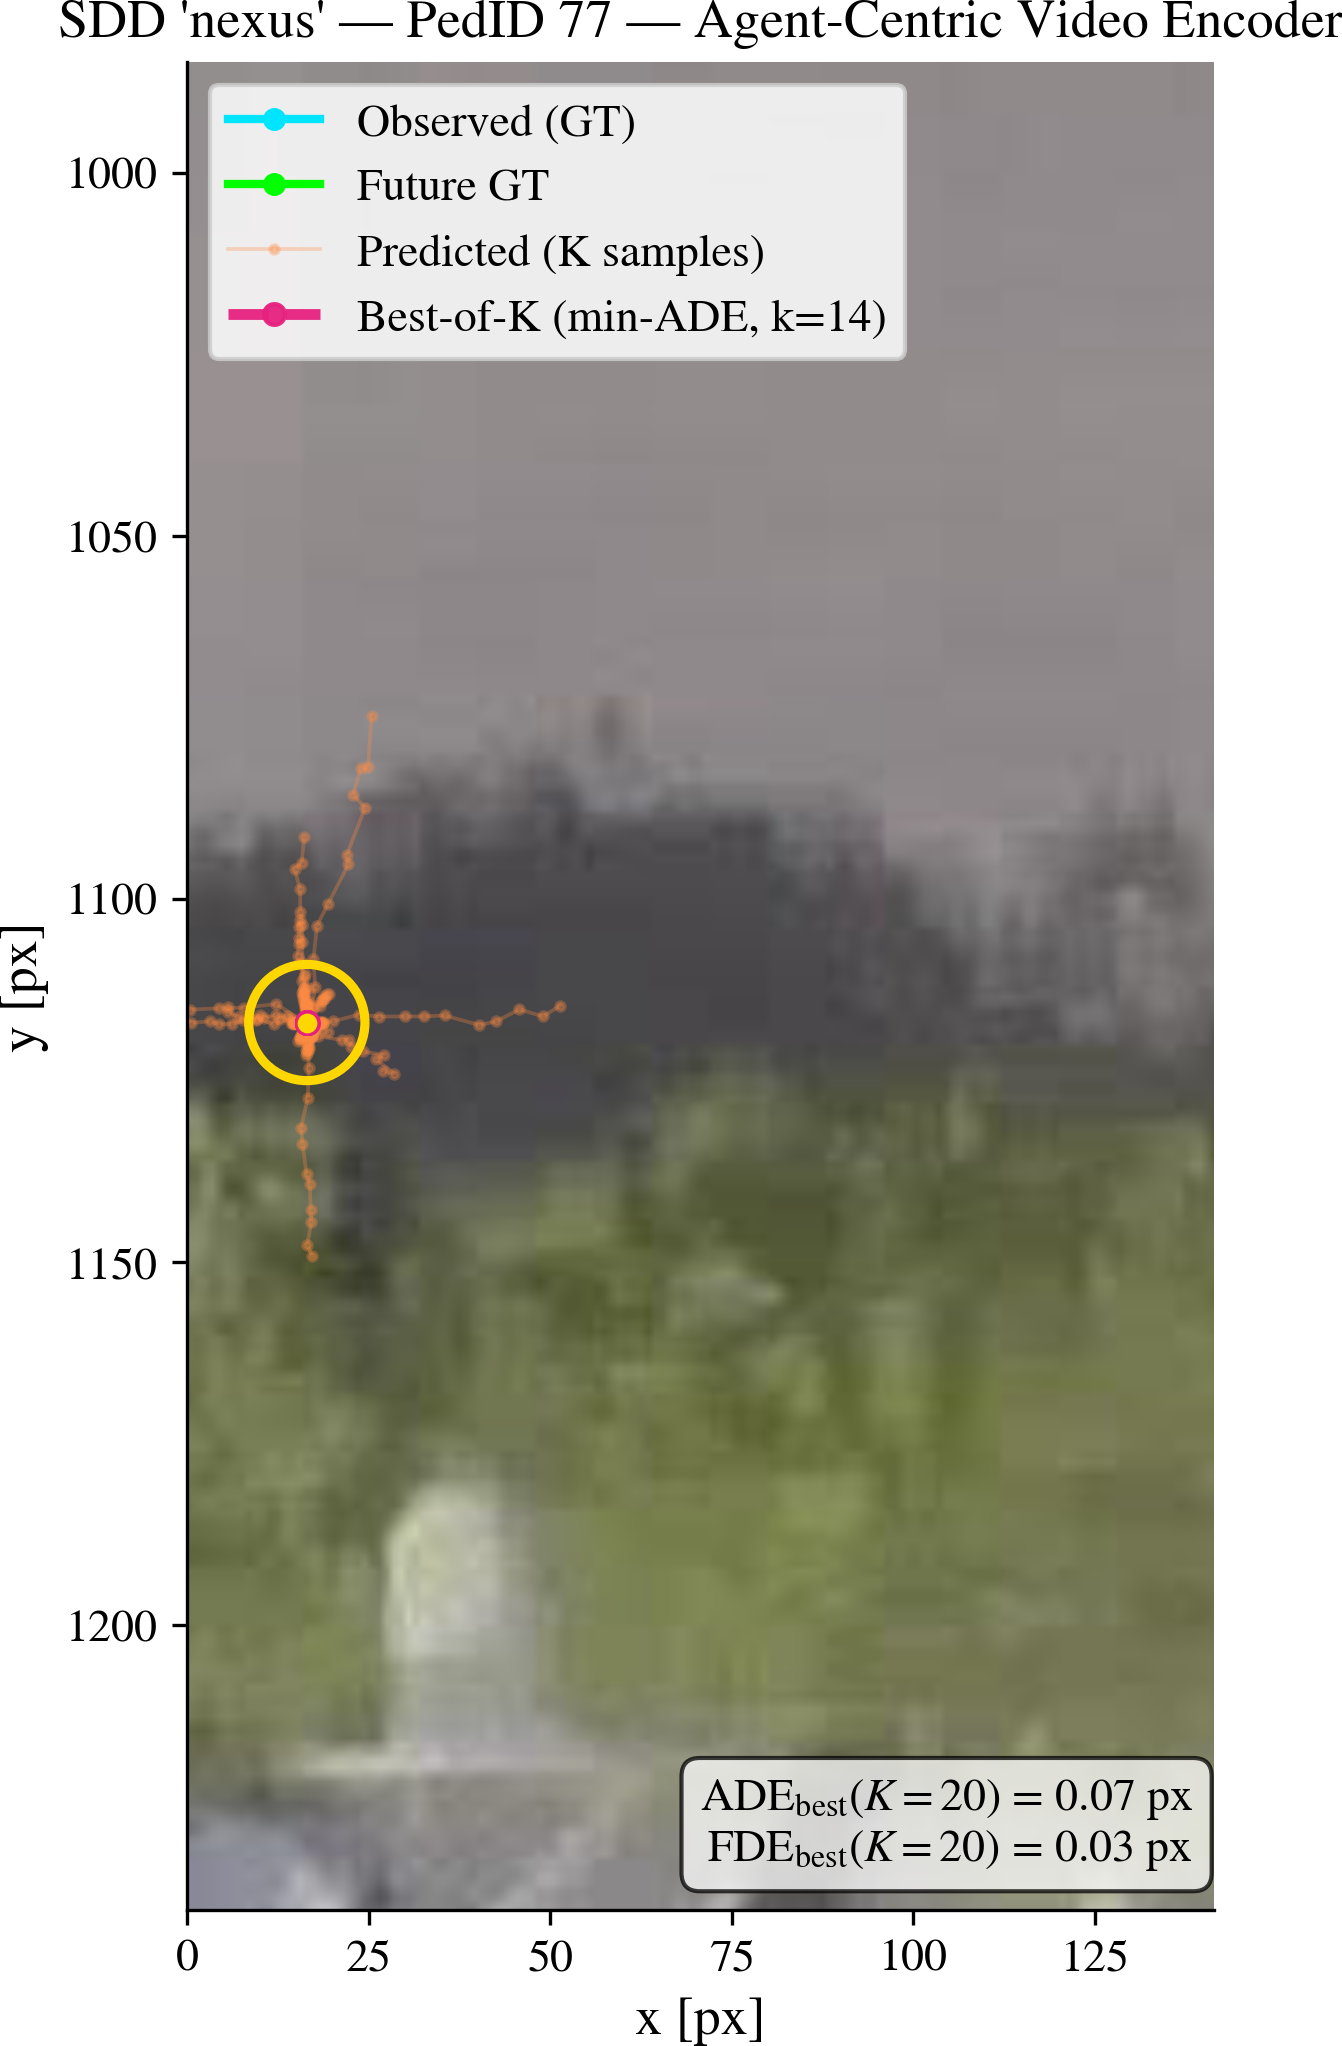
\includegraphics[width=0.32\textwidth]{figures/nexus_ped77_video9_f2519_agent_centric.png}
    \caption{Qualitative comparison on a nexus window: no-video vs.\ global vs.\
    agent-centric conditioning. In this vehicle-dense scene the agent-centric
    branch is the one that keeps the predicted futures closest to the observed
    target. \label{fig:nexus}}
\end{figure}

% -----------------------------------------------------------------------------
\section{Conclusion and Next Steps}
\label{sec:conclusion}

The two video-conditioning extensions of the MoFlow Teacher have been
implemented and evaluated on SDD. Global scene conditioning delivers a robust
reduction of average error and variance, while agent-centric conditioning shows
a complementary and promising improvement of best-of-$K$ behaviour whose source
still needs to be understood. The following actions are planned:

\begin{enumerate}
    \item \textbf{Formalise the scene-complexity correlation}: the measured
          density, interaction and obstacle statistics of
          Section~\ref{sec:interpretation} should be related quantitatively to
          the per-scene gains (e.g.\ linear regression of the error reduction
          against crowd density and non-pedestrian activity) to confirm the
          qualitative narrative with statistics.
    \item \textbf{Strengthen the ablations}: train the Global and Agent-Centric
          variants under a small hyper-parameter sweep (hidden dimension,
          dropout, crop size, number of frozen backbone blocks) and over
          several seeds, to assess the stability of the observed effects.
    \item \textbf{Improve the agent-centric branch}: relax the identity mask to a
          neighbour-aware local context, add optical-flow/frame-difference
          inputs for short-term visual motion, and make crop extraction robust
          to homography error (e.g.\ multi-scale crops).
    \item \textbf{Distill the best video-conditioned Teacher into a one-step
          IMLE Student.} All reported results concern the Teacher; the
          end-goal remains a video-conditioned Student that preserves the
          visual gains while restoring MoFlow's 100$\times$ faster sampling.
    \item \textbf{Prepare qualitative case studies} for direction changes and
          obstacle interactions, comparing no-video vs.\ video-conditioned
          futures against the ground truth.
\end{enumerate}

\end{document}
